\documentclass[12pt, a4paper]{article}

\setcounter{tocdepth}{4}
\setcounter{secnumdepth}{4}

% Avoid useless warnings about included images
% Reference: https://tex.stackexchange.com/a/78020
%\pdfsuppresswarningpagegroup=1

% Use \hypersetup here to get rid of the ugly boxes around links
\usepackage{hyperref}
\hypersetup{
  colorlinks=true,
  linkcolor=blue,
  urlcolor=blue
}

% Avoid warning about missing font for \textbackslash character.
\usepackage[T1]{fontenc}

% For nicer paragraph spacing
\usepackage{parskip}

\usepackage[disable]{todonotes}
%\usepackage{todonotes}

\usepackage{amsmath}%
\usepackage{amsfonts}%
\usepackage{amssymb}%
\usepackage{mleftright}
\usepackage{graphicx}
%\usepackage[miktex]{gnuplottex}
%\ShellEscapetrue
\usepackage{epstopdf}
\usepackage{longtable}
\usepackage{floatrow}
\usepackage{makecell}

% Use \setminted here to get horizontal line above and below listings
\usepackage{minted}
\setminted{
   frame=lines,
   framesep=2mm
}

\usepackage{textcomp}
\usepackage{color,soul}
\usepackage[font={small,it}]{caption}
\floatsetup[listing]{style=Plaintop}    
\floatsetup[longlisting]{style=Plaintop}    

% Turn off indentation but allow \indent command to still work.
\newlength\tindent
\setlength{\tindent}{\parindent}
\setlength{\parindent}{0pt}
\renewcommand{\indent}{\hspace*{\tindent}}

\addtolength{\textwidth}{0.8in}
\addtolength{\oddsidemargin}{-.4in}
\addtolength{\evensidemargin}{-.4in}
\addtolength{\textheight}{1.6in}
\addtolength{\topmargin}{-.8in}

\usepackage{longtable,supertabular}
\usepackage{listings}
\lstset{
  frame=top,frame=bottom,
  basicstyle=\ttfamily,
  language=XML,
  tabsize=2,
  belowskip=2\medskipamount
}

% All listings have a left aligned caption. This looks better as the listings themselves are left aligned.
\captionsetup[listing]{justification=justified,singlelinecheck=false}

\usepackage{tabu}
\tabulinesep=1.0mm
\restylefloat{table}

\usepackage{siunitx}
\usepackage{tablefootnote}
\usepackage{multirow}
\usepackage{colortbl}
\usepackage{footmisc}
\newenvironment{longlisting}{\captionsetup{type=listing}}{}
%\usepackage[colorlinks=true]{hyperref}

% Inline code fragments can run over the page boundary without ragged right.
\AtBeginDocument{\raggedright}

\newcommand{\UserGuide}{}

% Unconditional expectation operator
\DeclareMathOperator{\E}{\mathbb{E}}
\newcommand\Ex[1]{\E\mleft[\,#1\,\mright]}

% Conditional expectation operator
\newcommand\CEx[2]{\E\mleft[\,#1\;\middle|\;#2\,\mright]}

% Unconditional variance operator
\DeclareMathOperator{\V}{\mathbb{V}}
\newcommand\Var[1]{\V\mleft[\,#1\,\mright]}

\renewcommand\P{\ensuremath{\mathbb{P}}}
%\newcommand\E{\ensuremath{\mathbb{E}}}
\newcommand\Q{\ensuremath{\mathbb{Q}}}
\newcommand\I{\mathds{1}}
\newcommand\F{\ensuremath{\mathcal F}}
%\newcommand\V{\ensuremath{\mathbb{V}}}
\newcommand\YOY{{\rm YOY}}
\newcommand\Prob{\ensuremath{\mathbb{P}}}
\newcommand{\D}[1]{\mbox{d}#1}
\newcommand{\NPV}{\mathit{NPV}}
\newcommand{\CMS}{\mathit{CMS}}
\newcommand{\CDS}{\mathit{CDS}}
\newcommand{\CVA}{\mathit{CVA}}
\newcommand{\DVA}{\mathit{DVA}}
\newcommand{\FVA}{\mathit{FVA}}
\newcommand{\COLVA}{\mathit{COLVA}}
\newcommand{\FCA}{\mathit{FCA}}
\newcommand{\FBA}{\mathit{FBA}}
\newcommand{\KVA}{\mathit{KVA}}
\newcommand{\MVA}{\mathit{MVA}}
\newcommand{\PFE}{\mathit{PFE}}
\newcommand{\EE}{\mathit{EE}}
\newcommand{\EPE}{\mathit{EPE}}
\newcommand{\ENE}{\mathit{ENE}}
\newcommand{\EEPE}{\mathit{EEPE}}
\newcommand{\EEE}{\mathit{EEE}}
\newcommand{\EAD}{\mathit{EAD}}
\newcommand{\PE}{\mathit{PE}}
\newcommand{\NE}{\mathit{NE}}
\newcommand{\RC}{\mathit{RC}}
\newcommand{\RW}{\mathit{RW}}
\newcommand{\NS}{\mathit{NS}}
\newcommand{\PD}{\mathit{PD}}
\newcommand{\LGD}{\mathit{LGD}}
\newcommand{\DIM}{\mathit{DIM}}
\newcommand{\IM}{\mathit{DIM}}
\newcommand{\DF}{\mathit{DF}}
\newcommand{\MA}{\mathit{MA}}
\newcommand{\SCVA}{\mathit{SCVA}}
\newcommand{\bs}{\textbackslash}
\newcommand{\REDY}{\color{red}Y}
\newcommand{\IA}{\mathit{IA}}
\newcommand{\Th}{\mathit{TH}}
\newcommand{\CSA}{\mathit{CSA}}
\newcommand{\BACVA}{\mathit{BA-CVA}}
\newcommand{\MPR}{\mathit{MPR}}
\newcommand{\MF}{\mathit{MF}}
\newcommand{\RWA}{\mathit{RWA}}
\newcommand{\SNH}{\mathit{SNH}}
\newcommand{\HMA}{\mathit{HMA}}
\newcommand{\IH}{\mathit{IH}}
\newcommand{\Hdg}{\mathit{Hdg}}
\newcommand{\WS}{\mathit{WS}}
\newcommand{\FP}{\mathit{FP}}
\newcommand{\flt}{\mathit{flt}}
\newcommand{\fix}{\mathit{fix}}
\newcommand{\form}{\mathit{form}}
\newcommand{\OIS}{\mathit{OIS}}
\newcommand{\ON}{\mathit{ON}}
\newcommand{\AVG}{\mathit{AVG}}
\newcommand{\MAX}{\mathit{MAX}}
\newcommand{\MIN}{\mathit{MIN}}



\begin{document}

\title{ORE Intraday Option Valuation}
\date{11 November 2026}
\maketitle

\newpage

\section*{Document History}

\begin{center}
\begin{supertabular}{|l|l|p{8cm}|}
\hline
Date & Author & Comment \\
\hline
November 2026 & Dr. Marco Craveiro & initial version\\
\hline
\end{supertabular}
\end{center}

\newpage

\tableofcontents

\newpage

%-------------------------------------------------------------------------------
\section{Introduction}
%-------------------------------------------------------------------------------

\subsection{The Problem}\label{sec:problem}

QuantLib, and therefore ORE, measures time in whole days by default. An option that expires at 16:00 on the valuation
date has a time to expiry of zero, whatever the time of the valuation. Depending on the setting of
\texttt{includeReferenceDateEvents}, ORE then treats an ATM call expiring today as expired, with NPV zero, or prices it
at intrinsic value with delta 0.5 and gamma zero. Neither is usable: an ATM option one hour before its cut has the
largest gamma of its life.

\subsection{Motivation: ORE Studio}\label{sec:orestudio}

The work is motivated by ORE Studio \cite{orestudio}, a graphical front end for ORE. ORE Studio provides a database
backed user interface for configuring and running ORE, with persistent storage of inputs and outputs, and runs ORE on a
compute grid: each node runs a packaged \texttt{ore} executable against the inputs of a job. The bulk of the
quantitative work stays in ORE and QuantLib.\footnote{There are exceptions, mainly related to market data, and intraday time weighting is one of them. The time-weighted volatilities for today's expiries are computed by a process outside ORE, and ORE prices from them as from any other market data (\textit{c.f.} section \ref{sec:decay}).}

ORE Studio needs a headline report of the positions and sensitivities of options that expire on the valuation date,
run several times through the day. Its use of ORE sets the requirements that shape the approach of this document:

\begin{itemize}
\item \textbf{Two engines side by side.} The regular reports keep running on the regular build. The same day options
  report runs on a separate intraday build, packaged and deployed to the grid alongside it (\textit{c.f.} section
  \ref{sec:scope}).
\item \textbf{One trade representation.} ORE Studio generates the same portfolio XML whichever engine a report targets,
  and the XML must validate against the schema of the regular engine, which does not change.
\item \textbf{Conventions applied before ORE.} ORE Studio books the trades and assembles the market data. It converts
  each option's cut to a UTC timestamp (\textit{c.f.} section \ref{sec:timezones}), and produces the time-weighted volatilities as market data
  snapshots stamped with the valuation time (\textit{c.f.} section \ref{sec:decay}). ORE prices from timestamps and market data, with
  no knowledge of business centres or time weighting models.
\end{itemize}

Evidence from running the same day options report in ORE Studio will be added once the intraday build is packaged for
the grid. The examples of section \ref{sec:examples} stand in for it until then.

\subsection{Scope of the Same Day Options Report}\label{sec:scope}

The report values options that expire on the valuation date at an intraday asof. All other trades are valued by the
regular valuation at day resolution, where nothing changes.

\subsubsection*{In Scope}

\begin{itemize}
\item European vanilla options on equity, FX and commodity underlyings. Gamma grows as $1/\sqrt{T}$ into the cut.
\item Digital options expiring today. Delta and gamma near the strike are larger still and depend directly on the
  remaining volatility.
\item Barrier and touch options expiring today. The probability of a hit in the remaining hours depends on intraday
  volatility.
\item American options expiring today, priced with a finite difference engine on a very small time to expiry.
\end{itemize}

\subsubsection*{Out of Scope}

\begin{itemize}
\item Linear and rates products, such as interest rate and OIS swaps, FX and equity forwards and bonds. Their value
  does not depend on the volatility over the remaining hours.
\item Variance and volatility swaps, including those maturing today. They are forwards on realised variance or
  volatility, settled in cash; ORE represents a volatility swap as an \texttt{EquityVarianceSwap} with moment type
  \texttt{Volatility}. A swap maturing today is live until its final observation, such as the SP5 close, not only
  until the start of the day, and has an NPV that past returns mostly determine. On the last day only one return of
  the observation period, typically 21 to 252 returns, is still open, so the remaining volatility and gamma risk is
  small next to a same day ATM option. Their pricing engine also does not handle an intraday asof, see section
  \ref{sec:lim-varswap}.
\item Options that expired earlier today. Past its cut an option carries no volatility or gamma risk. A cash settled
  option in the money is worth its payoff until paid, which needs the settlement fixing at the cut time, see section
  \ref{sec:marketdata}.
\end{itemize}

\subsection{Contribution and Structure}\label{sec:contribution}

The work described here extends this material. It leaves QuantLib unchanged, and it changes no pricing model or
engine in ORE: options are valued by the existing engines, with the remaining time to expiry. The changes to ORE are
in how it reads its inputs and builds its market: date input, the expiry cut of a trade, and the pillars of FX
volatility surfaces. For existing inputs at day resolution and with tenor expiries, they leave results unchanged. The
work consists of

\begin{enumerate}
\item building ORE with the existing option and establishing that the resulting build is stable (\textit{c.f.} section
  \ref{sec:stability});
\item extending ORE's date input to accept a time of day and a UTC offset (\textit{c.f.} section \ref{sec:dateinput}), and reading an
  optional expiry cut time from a trade's envelope (\textit{c.f.} section \ref{sec:timezones});
\item letting FX volatility quotes carry an expiry date or datetime, so that FX surfaces can have a pillar at a cut,
  as equity surfaces already can (\textit{c.f.} section \ref{sec:fxfix});
\item a model of market data at an intraday asof, covering snapshots, fixings, volatility pillars at a cut and
  intraday time weighting (\textit{c.f.} sections \ref{sec:mktdata} and \ref{sec:decay}), with configuration for running the report,
  examples and an account of the limitations found (\textit{c.f.} sections \ref{sec:setup} to \ref{sec:limitations}).
\end{enumerate}

Section \ref{sec:stateofart} reviews the existing work on which this builds, and where it falls short for same day
options. Sections \ref{sec:build} to \ref{sec:decay} develop the approach in order of dependency: intraday dates, the
treatment of time and cuts, the model of market data at an intraday asof, and intraday time weighting. Section
\ref{sec:setup} turns this into configuration for running the report, section \ref{sec:examples} demonstrates it on
examples, section \ref{sec:limitations} lists the limitations found, and section \ref{sec:conclusion} concludes.

\paragraph*{Use of AI tools.}\label{sec:aiuse} Claude Code, an AI coding assistant, running the Claude Opus 5.5 model, was used in
the analysis of the problem, in the implementation of the changes to ORE and of the examples, and in the preparation of
this document. The author has reviewed the implementation in detail and has an understanding of all the work carried
out, and every result reported here was produced by running the code and examples described. Nevertheless, there
remains a risk that some aspects of the work were not completely understood, and readers should treat the results
accordingly.

%-------------------------------------------------------------------------------
\section{State of the Art}\label{sec:stateofart}
%-------------------------------------------------------------------------------

Three pieces of existing work bear on intraday valuation in ORE: QuantLib's high resolution dates, which give time a
resolution finer than a day; ORE's intraday power framework, which prices quantities within a day while keeping dates
at day resolution; and ORE's FX volatility surfaces, whose handling of expiries limits what a same day options report
can do for FX.

\subsection{QuantLib: High Resolution Dates}\label{sec:sota-ql}

Date handling in QuantLib \cite{quantlib} rests on the \texttt{Date} class, which by default stores a serial day
number. Day counters compute year fractions from pairs of dates, and term structures, volatility surfaces and pricing
engines convert dates to times through them. ORE \cite{ore} inherits this representation. Time is therefore measured in
whole days throughout, which suits almost every valuation but not an option in the last day of its life.

In 2015 QuantLib gained an alternative representation, selected at compile time by \texttt{QL\_HIGH\_RESOLUTION\_DATE}
and off by default \cite{qlhighres}. It stores a date as a \texttt{boost::posix\_time::ptime} with microsecond
resolution, behind the same interface as the serial number representation. With it

\begin{itemize}
\item dates can carry a time of day, \texttt{Date(d, m, y, hh, mm, ss, ms, us)},
\item \texttt{daysBetween()} returns fractional days, so the actual day counters (Actual/365 Fixed, Actual/360,
  Actual/Actual) return fractional year fractions within a day,
\item time series and index fixings can be keyed at any resolution.
\end{itemize}

Since day counters, term structures and pricing engines see dates only through this interface, they acquire intraday
resolution without modification. QuantLib exercises the mode in its continuous integration, which runs the test suite
in an intraday configuration, and in dedicated tests, among them a test of day counters within a day and a finite
difference Heston test that checks gamma as expiry approaches.

\paragraph*{What we take.} We take the representation unchanged. ORE is built with the option, and the day counters, term
structures, volatility surfaces and pricing engines of QuantLib and ORE are used as they are, so that the time to
expiry of an option becomes the remaining time without any change to pricing code. We also rely on QuantLib's own
testing of the mode, and add evidence that ORE built on it is stable (\textit{c.f.} section \ref{sec:stability}). What QuantLib does
not provide is a way to express a time of day in ORE's inputs; that is where our extension lies (\textit{c.f.} section
\ref{sec:dateinput}).

\subsection{ORE: Intraday Power}\label{sec:intradaypower}

ORE's intraday power framework prices power products that deliver in parts of a day, such as the 09:00 to 10:00
hour. It works in the default build, at day resolution. A commodity curve gives the price for each day, and intraday
shape factors, loaded as market data through the curve configuration, distribute it over the buckets of the day; they
can mix granularities, such as 15 minute buckets near term and hourly buckets further out, and carry their own
sensitivity and stress keys. A trade's load profile states which buckets it delivers into. The time of day is held
next to the date, as the start and end of a bucket in seconds from midnight. Historical fixings are named per bucket,
for example \texttt{POWER-PJM\_WH\_RT\_PK-2021-06-01-32400-36000} for 09:00 to 10:00, and the extra hour when clocks go
back carries a \texttt{-DST} suffix. On the valuation date a bucket with a published fixing is taken from the history
and a bucket without one is forecast, so the framework never needs the time of the valuation. Each curve has a
location for daylight saving. The framework's documentation is assembled from fragments of the User Guide, which the
product catalogue, the market data chapter and the parameterisation chapters include as well.

\paragraph*{What we take.}

\begin{itemize}
\item \textbf{Fixings at different times kept apart by name.} Each fixing source is its own index with a daily
  series, as each power bucket has its own name, so fixings taken at different times of day are never mixed (\textit{c.f.}
  section \ref{sec:marketdata}).
\item \textbf{The rule for the valuation date.} A fixing that has been published is used and one that has not is
  forecast; earlier dates require the fixing. The rule is robust when publication lags the cut and does not
  depend on the asof time.
\item \textbf{A template for the intraday profile.} If intraday time weighting is later computed inside ORE, the intraday
  shape term structure is the model for the variance weights, with buckets in seconds from midnight, mixed granularity
  and its own risk factor keys.
\item \textbf{The documentation structure.} As the feature matures, reference material such as the date input format
  and the setup of an intraday run moves into User Guide fragments in the same way.
\end{itemize}

\paragraph*{Where we differ.} Table \ref{tab:comparison} summarises the differences.

\begin{table}[H]
\centering
\begin{tabular}{|>{\raggedright\arraybackslash}p{3cm}|>{\raggedright\arraybackslash}p{5.5cm}|>{\raggedright\arraybackslash}p{5.5cm}|}
\hline
 & Intraday power & Intraday options \\
\hline
Date resolution & day, in the default build & microseconds, in a separate build \\
\hline
Time of day & seconds from midnight next to the date & part of the date \\
\hline
Intraday fixings & one name per bucket and day & one daily index per fixing source \\
\hline
Valuation date & published buckets used, others forecast & same rule, planned \\
\hline
Time zones & location per curve, for daylight saving & UTC timestamps, cuts converted outside ORE \\
\hline
Intraday profile & shape factors as market data in ORE & intraday time weighting outside ORE \\
\hline
Documentation & User Guide fragments & standalone document \\
\hline
\end{tabular}
\caption{Intraday power and intraday options compared}
\label{tab:comparison}
\end{table}

\begin{itemize}
\item \textbf{Date resolution.} A power price is linear in its bucket fixings: the time of day selects which prices
  apply but never enters a year fraction, so encoding the bucket next to the date is enough. An option's value depends
  on its time to expiry non-linearly, through $\sigma\sqrt{T}$, and that time is computed by the day counters of the
  curves, volatility surfaces and engines across QuantLib and ORE. The time of day must be part of the date for all of
  them to see it, which requires \texttt{QL\_HIGH\_RESOLUTION\_DATE}, at the cost of a second build.
\item \textbf{Intraday fixings.} Power buckets lie on a fixed grid set by the load profile, so a name per bucket and
  delivery date is natural. Option settlement fixings are taken by fixing sources at their cuts, so they are named by
  source, as ORE's FX indices already are, with one daily series per source. Both approaches keep fixings taken at
  different times apart by name and stay at day resolution.
\item \textbf{Time zones.} All buckets of a power market are in that market's local time, so a location per curve is
  enough. The cut of an option is set by a business centre that may differ from the underlying's market and from the
  booking location, and expiries in several centres must be compared with one asof. The booking system therefore
  converts every cut to UTC (\textit{c.f.} section \ref{sec:timezones}).
\item \textbf{Intraday profile.} The intraday profile of an option is the time weighting of its volatility. It is kept outside
  ORE (\textit{c.f.} section \ref{sec:decay}): the choice of time weighting model belongs with the process that keys the volatilities, and ORE
  prices from any time-weighted volatilities it is given.
\end{itemize}

\subsection{ORE: FX Volatility Surfaces}\label{sec:sota-fx}

ORE builds an FX volatility surface for a currency pair from market quotes of the form
\texttt{FX\_OPTION/RATE\_LNVOL/<CCY1>/<CCY2>/<expiry>/<strike>}. The strike is ATM, a delta such as 25 delta call or
put, or a risk reversal or butterfly. The curve configuration chooses the shape of the surface: an ATM curve, or a smile
built from delta quotes, from risk reversals and butterflies, by vanna-volga, or from absolute strikes. It lists the
expiries explicitly, or takes them from the market data by wildcard for ATM, delta and risk reversal and butterfly
surfaces. A surface built from risk reversals and butterflies can weight the time between pillars with the
\texttt{FxOptionTimeWeighting} convention, which gives weekdays, trading centres and events their own weights in whole
days.

The expiry of an FX option quote is a tenor, and only a tenor. The quote stores it as a period, and the market data
parser reads it with a period parser, so a quote with a date expiry is rejected when it is read. The surface turns each
tenor into a pillar date by advancing the asof by the tenor on the curve's calendar, with the following business day
convention and no spot lag. The ATM curve does not enforce monotone total variance: it is built with decreasing variance
allowed between pillars.

Equity and commodity volatilities differ on exactly this point. Table \ref{tab:volexpiries} compares the three asset
classes.

\begin{table}[H]
\centering
\small
\begin{tabular}{|l|>{\raggedright\arraybackslash}p{3.6cm}|>{\raggedright\arraybackslash}p{3.0cm}|>{\raggedright\arraybackslash}p{2.6cm}|>{\raggedright\arraybackslash}p{2.0cm}|}
\hline
Asset class & Quote expiry & Tenor to pillar & Pillar at a cut & Monotone variance \\
\hline
Equity & date or tenor & asof plus tenor, adjusted & yes, tested & enforced \\
\hline
Commodity & date, tenor or future continuation & asof plus tenor, adjusted & yes, tested & enforced \\
\hline
FX & tenor only & asof advanced by tenor on the calendar & no & not enforced \\
\hline
\end{tabular}
\caption{Volatility quote expiries by asset class, with FX as before the extension of section \ref{sec:fxfix}}
\label{tab:volexpiries}
\end{table}

For a same day option the consequence is direct. Its expiry lies before the first pillar of the surface, so it takes
the volatility of that pillar, held flat. Before the extension of section \ref{sec:fxfix}, the SameDayInstruments
example (\textit{c.f.} section \ref{sec:ex-instruments}) priced its EURUSD call expiring at 15:00 UTC at 12.1699\% at every
asof from 09:00 to 14:55: the volatility of the 1M pillar, the first in the shared configuration. The pricing itself is right, with the exact time to the cut, but the
volatility is not one that anyone keyed for today. Three things follow:

\begin{itemize}
\item \textbf{No volatility for a cut.} No quote can carry the volatility of today's 15:00 UTC cut, so the booking
  system has no way to supply it, time-weighted or not.
\item \textbf{One volatility for all of today's cuts.} Options expiring at the Tokyo, ECB and New York cuts of the same
  day all take the same volatility.
\item \textbf{No adequate workaround.} The shortest tenor, 1D, lies a day after the asof. A time-weighted volatility put
  there would apply to every expiry before the same time tomorrow, including tomorrow's morning cuts, and would still
  give one volatility per pair for the whole day.
\end{itemize}

Same day options on FX are therefore priced with the right time and the wrong volatility, and intraday time weighting cannot
be applied to them. Since FX options are a large part of any same day options book, this is the main gap in ORE for the
report.

\paragraph*{What we take.} We keep the FX surfaces as they are: their quote types and strikes, their shapes, their
mapping from tenors to pillar dates, their interpolation and their time weighting. For expiries we take the approach
of ORE's equity and commodity volatility surfaces. Their quotes already accept an expiry date as well as a tenor, the
equity quote as a date or period and the commodity quote through ORE's \texttt{Expiry} type, and their curves build
pillars from such dates alongside tenors, dropping a pillar at or before the asof. An expiry date given with a time of
day in the intraday build is then a pillar at a cut, as the equity example of section \ref{sec:ex-decay} shows. What
is missing for FX is exactly this: an FX quote cannot carry an expiry date, so its surface cannot build such a pillar.
Section \ref{sec:fxfix} extends FX in the same manner.

%-------------------------------------------------------------------------------
\section{Intraday Dates}\label{sec:build}
%-------------------------------------------------------------------------------

QuantLib's high resolution dates (\textit{c.f.} section \ref{sec:sota-ql}) are the foundation. This section builds ORE on
them, establishes that the result is stable, and describes how dates with a time of day are written.

\subsection{Building ORE}

ORE is built with the option on as follows:

\begin{minted}[fontsize=\footnotesize]{text}
cmake -S . -B build/<preset>-intraday -G Ninja -DCMAKE_BUILD_TYPE=Release \
      -DQL_HIGH_RESOLUTION_DATE=ON <usual options>
\end{minted}

The intraday build is intended for a same day options report only, see section \ref{sec:scope}. All other valuation
stays on the regular build at day resolution.

\subsection{Stability}\label{sec:stability}

The following checks were run against ORE v1.8.17.0, built with clang in release mode.

\begin{itemize}
\item QuantLib, QuantExt, OREData, OREAnalytics, the application and the test suites compile without errors.
\item The QuantExt and OREAnalytics unit test suites pass. The OREData suite passes except for four derived schedule
  tests, which fail in the default build too.
\item With every date at midnight the intraday build behaves like the default build, because year fractions, serial
  numbers and comparisons are identical. Legacy Example 22 (equity, FX and swaption options, NPV and sensitivity)
  reproduces the expected output shipped with the source: NPVs are identical, sensitivities are identical, cashflows
  and curves agree to a relative difference of $3\cdot 10^{-14}$.
\item Every date operation goes through \texttt{ptime}. Example 22 ran roughly 25 to 35\% slower than on a default
  build at an earlier source version, so the figure is indicative only. For a report over a small portfolio the
  overhead does not matter.
\end{itemize}

\subsection{Date Input}\label{sec:dateinput}

In an intraday build every date in ORE input can carry a time of day in ISO 8601 form,
\texttt{<date>T<HH:MM[:SS[.ffffff]]>}, where \texttt{<date>} is any date format ORE accepts, for example
\texttt{2016-02-05T15:00} or \texttt{2016-02-05T15:00:30.25}. This covers the asof date, market data and fixings,
which are inputs of a run. Trade XML keeps its dates plain and gives an option's expiry time as an
\texttt{ExpiryCutTime} in the trade's envelope (\textit{c.f.} section \ref{sec:timezones}). Times are UTC. A datetime may end in \texttt{Z} or a UTC offset, for example \texttt{2016-02-05T16:00-05:00},
which ORE converts to UTC on reading, here 21:00. A datetime without either is taken as UTC. In a default build a
datetime fails with an error naming \texttt{QL\_HIGH\_RESOLUTION\_DATE}. See section \ref{sec:timezones}.

%-------------------------------------------------------------------------------
\section{Time and Cuts}\label{sec:timezones}
%-------------------------------------------------------------------------------

With dates that carry a time, the question is which time an option expires at, and on which clock.

\subsection{Requirement}

The expiry time of an option is defined relative to a business centre, not as an absolute time. FX options expire at a
named cut, such as 10:00 New York or 15:00 Tokyo, whatever the currency pair. An equity index option expires at the
close of its exchange, such as 16:00 New York. A valuation at an intraday asof has to compare the asof and the expiry on
one clock, and the offset of each business centre from UTC changes with daylight saving, on dates that differ between
centres. Table \ref{tab:nycut} shows the same local cut at two different UTC times.

\begin{table}[hbt]
\centering
\begin{tabular}{|l|l|l|}
\hline
Date & Local cut & UTC \\
\hline
5 February 2016 & 16:00 New York & 21:00 \\
5 July 2016 & 16:00 New York & 20:00 \\
\hline
\end{tabular}
\caption{A New York cut in UTC, winter and summer}
\label{tab:nycut}
\end{table}

A naive time of day is therefore not sufficient: the asof and every expiry must be instants on one clock.

FpML, the industry standard for representing derivative trades, models the expiry of an FX option in the same terms
\cite{fpmlfxexercise}. An \texttt{expiryDate} is accompanied by an \texttt{expiryTime}, a local time of day
(\texttt{hourMinuteTime}) together with the business centre whose clock it refers to (\texttt{businessCenter}), and
optionally a \texttt{cutName} by which the time is known in the market. FpML recommends \texttt{expiryTime} in
preference to \texttt{cutName} as the formal definition of the expiry time. Its cut name scheme \cite{fpmlcutname}
lists the standard named cuts, among them:

\begin{table}[H]
\centering
\begin{tabular}{|l|l|l|}
\hline
FpML cut name & Local time & UTC on 5 February 2016 \\
\hline
\texttt{NewYork} & 10:00 New York & 15:00 \\
\texttt{ECB} & 13:30 London & 13:30 \\
\texttt{LondonEveningGold} & 15:00 London & 15:00 \\
\texttt{Comex} & 14:30 New York & 19:30 \\
\hline
\end{tabular}
\caption{Some standard cuts from the FpML cut name scheme, converted to UTC}
\label{tab:fpmlcuts}
\end{table}

Other cuts are market conventions outside the scheme, such as the Tokyo cut at 15:00 Tokyo time, 06:00 UTC, or the close
of an exchange, such as 16:00 New York for SP5, 21:00 UTC in winter.

\subsection{Backwards Compatibility}\label{sec:compat}

The intraday build runs alongside the regular build (\textit{c.f.} section \ref{sec:orestudio}), and both price trades from the same
portfolio XML. This constrains where the expiry time can go:

\begin{itemize}
\item \textbf{The regular build does not change.} Its schema, \texttt{xsd/ore\_types.xsd} and
  \texttt{xsd/instruments.xsd}, and its parser stay as they are. Its \texttt{date} type allows at most 10 characters,
  and its \texttt{parseDate} rejects a time of day.
\item \textbf{One portfolio XML.} The booking system generates the same XML whichever build a report targets.
  Generating different XML per build would tie every trade to a build version and multiply the representations to
  maintain.
\item \textbf{Schema validation.} The XML must validate against the unchanged schema. ORE's own check,
  \texttt{xsd/check.sh}, also validates every XML file of the examples with \texttt{xmllint}.
\end{itemize}

\subsection{Avenues Explored}

Table \ref{tab:cutavenues} lists the options considered for carrying the expiry time, and why each was kept or
rejected.

\begin{table}[H]
\centering
\small
\begin{tabular}{|>{\raggedright\arraybackslash}p{4.0cm}|>{\raggedright\arraybackslash}p{8.3cm}|l|}
\hline
Avenue & Assessment & Outcome \\
\hline
Naive time of day in the expiry & Cuts are set by business centres whose offset from UTC changes with daylight saving on
different dates. The asof and expiries in several centres cannot be compared on one clock. & rejected \\
\hline
Business centre and cut conventions in ORE, converted with time zone rules & Moves time zone rules, which change when
governments change them, into ORE. The booking system already knows each cut and can convert it. & rejected \\
\hline
Datetime in \texttt{ExerciseDate} & Fails the regular schema and the regular parser, so the booking system would have to
generate different XML per build. Also fails \texttt{xsd/check.sh} on the examples. & rejected \\
\hline
New \texttt{ExpiryCutTime} element in the option data, with a schema change & Follows the precedent of FpML, which
models expiration date and time separately, but the unchanged regular schema rejects the new element, so the XML would
again differ per build. & rejected \\
\hline
Separate input of cut times, by trade or underlying, read only by the intraday build & Keeps the trade XML unchanged,
but adds another build specific output for the booking system to produce and keep in step with the portfolio. & not
chosen \\
\hline
\texttt{ExpiryCutTime} in the envelope's additional fields & Valid under the unchanged schema, which accepts any content
there. The regular build ignores it; the intraday build reads it. One XML for both builds. & chosen \\
\hline
\end{tabular}
\caption{Avenues for carrying the expiry time}
\label{tab:cutavenues}
\end{table}

\subsection{Design}

All times in ORE are plain timestamps in UTC. ORE has no notion of business centres, cuts or daylight saving.

\begin{itemize}
\item \textbf{UTC internally.} Every datetime inside ORE is in UTC. A datetime in the input without a designator is in
  UTC.
\item \textbf{Offsets in the input.} A datetime may end in \texttt{Z} or a UTC offset, for example
  \texttt{2016-02-05T16:00-05:00}, which ORE converts to 21:00 UTC on reading. This applies to the asof and the market
  data, which are inputs of the run rather than of the trade.
\item \textbf{Cuts in the trade.} The trade keeps a plain \texttt{ExerciseDate}. The booking system converts the
  option's cut to UTC, applying the daylight saving rules of the business centre, and adds it as an
  \texttt{ExpiryCutTime} to the envelope's additional fields:
\begin{minted}[fontsize=\footnotesize]{xml}
<Envelope>
  <CounterParty>CPTY_A</CounterParty>
  <NettingSetId>CPTY_A</NettingSetId>
  <AdditionalFields>
    <ExpiryCutTime>21:00Z</ExpiryCutTime>
  </AdditionalFields>
</Envelope>
\end{minted}
  The format is \texttt{HH:MM[:SS[.ffffff]]}, followed by \texttt{Z} or a UTC offset; no designator means UTC. The
  intraday build applies the cut to every exercise date of the option. The regular build ignores it.
\item \textbf{No cut given.} A date only expiry on the valuation day would otherwise expire at midnight, at the start of
  the day. The intraday build treats it as expiring at the end of that day, 23:59:59 UTC, and logs a warning for the
  trade. Expiries on other days keep their meaning, so that the intraday build reproduces the regular build on day
  resolution inputs.
\item \textbf{Market data.} The asof and the market data snapshots are stamped in UTC.
\end{itemize}

The envelope route has one weakness: a misspelled field name is ignored rather than rejected. The warning for a same
day option priced without a cut makes such a case visible.

In the implementation, \texttt{OptionData} reads the cut when it is loaded: it walks up from its own XML node to the
enclosing \texttt{Trade} (or \texttt{SubTrade}) and reads \texttt{Envelope/AdditionalFields/ExpiryCutTime}. A
malformed cut, a cut with an \texttt{ExerciseSchedule} instead of \texttt{ExerciseDates}, and a cut on an exercise date
that already carries a time are rejected with an error naming the field. The cut and the default for the valuation day
are applied when the exercise dates are read, against the evaluation date at that moment, so all trade types that take
their expiry from \texttt{OptionData} pick them up without change. Writing a trade back to XML keeps the plain dates and
the envelope field. All of this is compiled only in the intraday build; the regular build neither reads nor validates
the field. The examples of section \ref{sec:examples} give their expiries this way, and their XML validates against
the unchanged schema.

This follows the same principle as intraday time weighting in section \ref{sec:decay}: conventions about time are applied
where the trades and market data are produced, and ORE prices from instants. It keeps time zone rules, which change
when governments change them, out of ORE, and lets ORE stay a pure consumer of timestamps. In FpML terms,
\texttt{ExpiryCutTime} is the \texttt{expiryTime} of the option, converted from its business centre to UTC by the
booking system.

%-------------------------------------------------------------------------------
\section{Market Data}\label{sec:mktdata}
%-------------------------------------------------------------------------------

This section describes the market data an intraday run consumes: one snapshot per asof, daily fixings, and
volatilities with a pillar at each of today's cuts, for every asset class.

\subsection{Asof and Snapshots}\label{sec:asofcuts}

The asof date carries the valuation time:

\begin{minted}[fontsize=\footnotesize]{xml}
<Parameter name="asofDate">2016-02-05T15:00</Parameter>
\end{minted}

Market data loaders look quotes up by the exact asof. The market data must therefore carry the same datetime as the
asof: an intraday run consumes a market snapshot stamped with its time. Quotes stamped with the date alone are not
found.

Two different times are involved, and both are UTC:

\begin{itemize}
\item \textbf{The asof} is the time at which the market is observed and the valuation is made. A run has a single
  asof, and every quote in its market data snapshot is stamped with it, whatever the quote refers to.
\item \textbf{A cut} is the time at which an option expires. It appears in two places only: as the expiry of a trade,
  through \texttt{ExpiryCutTime}, and as the expiry of the volatility pillar for that cut, in the name of the quote.
\end{itemize}

Market data has no time zone of its own: the stamp of a snapshot is the asof in UTC. A cut is never a property of the
market data as a whole, only of a quote's expiry.

\subsection{Daily and Intraday Fixings}\label{sec:marketdata}

Market data is daily by default: a fixing, payment date or schedule date for day $D$ applies to the whole of $D$. Only
three things carry a time of day: the asof, the expiry cut of a trade, and the expiry of a volatility pillar at a cut.

A fixing taken at a given time of day is identified by its source, not by a time stamp. ORE's FX indices already name
the source in the index, \texttt{FX-<TAG>-<CCY1>-<CCY2>}, for example \texttt{FX-ECB-EUR-USD}, and the intraday power
framework names each bucket (\textit{c.f.} section \ref{sec:intradaypower}). The settlement fixing of an option at a cut follows
the same pattern: each fixing source, such as a fixing at the New York cut or the London afternoon gold price, is its
own index with a daily series. One index never mixes fixings taken at different times, so a daily fixing is never
taken for another, and no series keyed by time of day is needed.

On the valuation date a fixing that has been published is used, and one that has not is forecast. For earlier dates
the fixing must be present. This is the rule the intraday power framework applies to its buckets, and it does not
depend on the time of the asof. ORE does not yet apply it consistently at an intraday asof (\textit{c.f.} sections
\ref{sec:lim-fixingdates} and \ref{sec:lim-todayfixing}).

\subsection{Volatility Pillars at a Cut}\label{sec:volpillars}

A volatility pillar at a cut lets a snapshot give each of today's expiries its own volatility.

Consider a day with options expiring at three cuts: the Tokyo cut at 06:00 UTC, the ECB cut at 13:30 UTC and the New
York cut at 15:00 UTC. The time weighting process keeps one intraday volatility series per underlying and cut. A snapshot at
12:00 UTC is stamped \texttt{2016-02-05T12:00Z} throughout and carries, for each cut, the value of its series at
12:00 as a quote whose expiry is the cut:

\begin{minted}[fontsize=\footnotesize]{text}
2016-02-05T12:00Z FX/RATE/EUR/USD                                       1.1135
2016-02-05T12:00Z FX_OPTION/RATE_LNVOL/EUR/USD/2016-02-05T13:30Z/ATM    0.0951
2016-02-05T12:00Z FX_OPTION/RATE_LNVOL/EUR/USD/2016-02-05T15:00Z/ATM    0.0968
2016-02-05T12:00Z FX_OPTION/RATE_LNVOL/EUR/USD/1M/ATM                   0.1012
\end{minted}

The Tokyo cut has passed by 12:00, and its series has ended. A quote for a cut at or before the asof is ignored by the
volatility curve, so a snapshot that still carries it does no harm, but the time weighting process need not publish it. An
option expiring at a cut is priced off the pillar at its own cut; an expiry between two pillars is interpolated in total
variance between them.

The series of different cuts are not independent. Total variance to the expiry must not fall from one cut to the next,
$\sigma_{\text{ECB}}^2\,\tau_{\text{ECB}} \le \sigma_{\text{NY}}^2\,\tau_{\text{NY}}$, since the difference is the
variance between the two cuts. Equity and commodity curves reject a snapshot that breaks this with the error
``variance must be non-decreasing''. FX curves do so when \texttt{EnforceMonotoneVariance} is set, and otherwise log a
warning (\textit{c.f.} section \ref{sec:fxfix}). The time weighting process must therefore weight the series of a day's cuts consistently,
for example from one set of intraday weights.

FX quotes with an expiry at a cut, as above, rely on the extension of section \ref{sec:fxfix}. The values above are
illustrative; the MultipleCutsFx example (\textit{c.f.} section \ref{sec:ex-multicuts}) runs this case with three cuts.

\subsection{FX Volatility Pillars}\label{sec:fxfix}

Section \ref{sec:sota-fx} shows that an FX volatility surface cannot have a pillar at a cut, because FX option quotes
take their expiry as a tenor only. This subsection describes the extension that removes the limitation, and the
examples of section \ref{sec:ex-multicuts} show it at work.

\subsubsection*{Requirements}

\begin{itemize}
\item \textbf{The same rule as other asset classes.} FX volatilities must accept a pillar at a cut in the same way as
  equity and commodity volatilities, so that same day options behave alike whatever the underlying.
\item \textbf{The intraday cases resolved.} A pillar at a cut, several cuts in a day with a volatility each, and
  time-weighted volatilities per cut, for ATM curves and for the delta and risk reversal and butterfly surfaces that take
  their expiries from the market data.
\item \textbf{The smallest change.} Existing inputs with tenor expiries give identical results. The public interface
  only gains functions, so existing users, including the Python bindings, are unaffected. No refactoring beyond what
  the extension needs.
\end{itemize}

\subsubsection*{Design}

\begin{itemize}
\item \textbf{Quotes.} An FX option quote holds its expiry as ORE's \texttt{Expiry} type, which commodity option quotes
  already use: a date or a tenor. The market data parser accepts
  \texttt{FX\_OPTION/RATE\_LNVOL/EUR/USD/2016-02-05T15:00Z/ATM} as well as \texttt{.../1M/ATM}. The existing
  constructor taking a tenor and the accessor \texttt{expiry()} returning it are unchanged for tenor quotes; a new
  constructor takes an \texttt{Expiry}, and a new accessor \texttt{optionExpiry()} returns it. The Python bindings,
  which expose only the tenor forms, need no change.
\item \textbf{Pillars.} The FX volatility curve turns each expiry into a pillar date with a single helper. A tenor keeps
  today's mapping exactly, advancing the asof by the tenor on the curve's calendar. A date or datetime is used as given.
  Pillars from tenors and dates are sorted together, and a pillar at or before the asof is dropped with a log message,
  as the equity volatility curve does. This applies to every surface the curve builds: ATM, vanna-volga, delta, risk
  reversal and butterfly, and absolute strikes, and to expiries taken by wildcard from the market data or listed in the
  configuration.
\item \textbf{One change in QuantExt.} The risk reversal and butterfly surface read no time shorter than one day, so a
  pillar at a cut returned the volatility at one day. Its minimum time is now the shorter of one day and the first
  pillar. Tenor pillars are never less than a day away, so results for tenor surfaces do not change.
\item \textbf{No build flag.} The extension is not specific to the intraday build. In the regular build FX quotes gain
  expiry dates; in the intraday build they also accept a time of day, because the date parser accepts one there.
\end{itemize}

\subsubsection*{Monotone Variance}

The FX ATM curve allows the total variance to decrease between pillars, unlike equity and commodity curves, which
reject it. With several cuts in a day, each with its own volatility, an inconsistent snapshot becomes easy to produce,
and a decreasing total variance means a negative forward variance between two cuts. Three measures address this:

\begin{itemize}
\item \textbf{A configuration option.} The FX volatility curve configuration gains an optional
  \texttt{EnforceMonotoneVariance} element. When it is true, a decreasing total variance makes the curve fail to build,
  as for equity and commodity. The ATM and vanna-volga surfaces apply it through QuantLib; the delta and risk reversal
  and butterfly surfaces have no such setting of their own, so the check is made on their ATM pillars.
\item \textbf{A warning otherwise.} The default is false, which keeps today's behaviour for existing configurations. A
  decreasing total variance between two pillars is then logged as a structured warning, ``Decreasing ATM total
  variance'', that names the curve and the two pillars.
\item \textbf{Validation before ORE.} ORE Studio checks that the published volatilities give non-decreasing total
  variance across a day's cuts before a snapshot reaches ORE.
\end{itemize}

\subsubsection*{Verification}

\begin{itemize}
\item \textbf{Unit tests.} Quotes with tenor, date and datetime expiries parse, and malformed ones are rejected. ATM,
  delta and risk reversal and butterfly surfaces built from mixed tenor and date pillars return each pillar's quoted
  volatility; pillars at or before the asof are ignored; two cuts on the asof's day return their own volatilities. A
  decreasing total variance fails to build when \texttt{EnforceMonotoneVariance} is set and logs the warning otherwise.
\item \textbf{Regression.} Legacy Example 22 and an FX smile example built from risk reversals and butterflies give
  identical FX results to the code before the change, and log no new warning.
\item \textbf{Examples.} The MultipleCuts examples (\textit{c.f.} section \ref{sec:ex-multicuts}) price options at three FX
  cuts, two equity cuts and two commodity cuts, each off its own pillar.
\end{itemize}

\subsubsection*{Out of Scope}

At a pillar at a cut, the risk reversal and butterfly surface returns the quoted ATM volatility at the delta neutral
strike to within $6\cdot 10^{-4}$ relative, because QuantExt rebuilds the smile with a settlement date counted in whole
days. The mapping from tenors to pillar dates differs between FX and equity, and stays as it is, since aligning it would
move existing pillars. The FX time weighting works in whole days, and its combination with pillars at a cut is not
addressed. A simulated volatility surface still cannot hold a pillar at a cut, for any asset class (\textit{c.f.} section
\ref{sec:lim-simvol}).

%-------------------------------------------------------------------------------
\section{Intraday Time Weighting}\label{sec:decay}
%-------------------------------------------------------------------------------

\subsection{Motivation}

Variance does not arrive evenly through the trading day. Activity, and with it variance, concentrates around the open,
the close and scheduled releases, and is low in quiet hours \cite{andersen1997, andersen1998}. A volatility keyed in the morning for an expiry later the
same day reflects the variance expected over all remaining hours, the busy ones included. As the busy hours pass, less
variance is left per remaining hour, so the volatility that prices the rest of the day has to fall. Measuring time in
weighted time, with a weight for each part of the day, captures this; it is called intraday time weighting
\cite{clark2011}. On trading desks the resulting fall of the volatility through the day is often called volatility
decay. This document uses the term of the literature, not least because the same weighting can also make the
volatility rise (\textit{c.f.} section \ref{sec:decay-formulation}).

Time weighting is often also used to compensate for systems that measure time in whole days, by inflating the volatility of
short dated options and reducing it as the day passes. With intraday date resolution the time to expiry is exact, so
in an intraday build time weighting only expresses uneven intraday variance.

\subsection{Formulation}\label{sec:decay-formulation}

Time is measured in variance time. Each interval of the day has a weight $w(u)$, and
\begin{equation}
\tau(t, T) = \int_t^T w(u)\, du
\end{equation}
is the weighted time from $t$ to the expiry $T$. Weighting time this way is standard practice for short dated
options; Clark gives sample day and intraday weights for EURUSD \cite{clark2011}. Over several days the same idea gives
weekends and holidays less weight than trading days \cite{moontower, globalcapital}, which ORE already supports at the
level of whole days for FX volatility surfaces through the \texttt{FxOptionTimeWeighting} convention. The intraday
weights here apply the idea within the day. The total variance keyed at the start of the day $t_0$ is kept, and
variance is removed as weighted time passes. The volatility that prices the remaining clock time $T - t$ is then
\begin{equation}
\sigma(t) = \sigma_0 \sqrt{\frac{\tau(t, T)}{\tau(t_0, T)} \cdot \frac{T - t_0}{T - t}}
\end{equation}

\begin{itemize}
\item With equal weights $\sigma(t) = \sigma_0$ and the volatility does not change.
\item With heavier weights early in the session the volatility falls through the busy period and then stays flat.
\item A scheduled event adds a lump $\epsilon_j$ of variance at time $e_j$. Variances of independent components add,
  so event variance adds to the background variance rather than to the volatility, and implied volatility rises
  before scheduled announcements and falls after them \cite{wright2020}. Once the event has passed its variance leaves
  $\tau$ and the volatility drops in a single step.
\end{itemize}

A simpler alternative is a linear decline in variance from a keyed opening volatility to a closing volatility. It does
not take into account where in the day the variance falls.

Variance time does not make the volatility fall in every case. The volatility for the rest of the day is set by the
average weight of the hours still to come, so it falls while busier than average hours pass, and rises while quieter
ones do. With activity concentrated early in the day it falls towards the cut. With a quiet night and a busy open and
close, the pattern reported for intraday markets \cite{andersen1997}, it rises through the quiet hours, drops once the
busy open has passed, and rises again into the busy close. Figure \ref{fig:volprofiles} shows both for the same keyed
volatility. The examples of this document use profiles under which the volatility falls.

\begin{figure}[H]
\centering
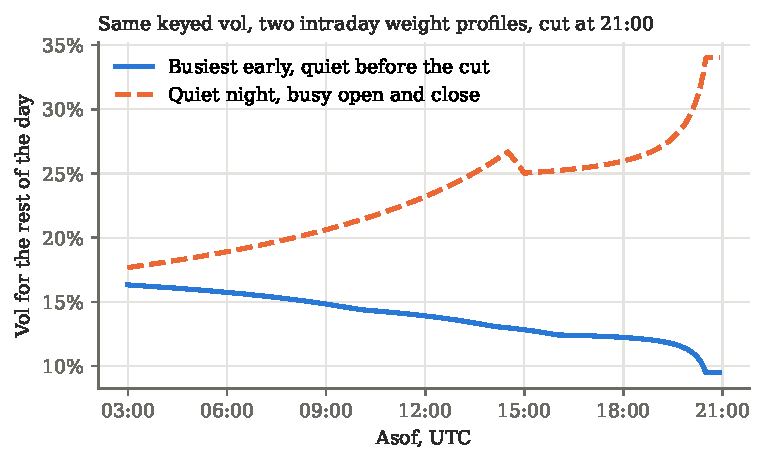
\includegraphics[width=0.85\textwidth]{pics/vol_profiles.pdf}
\caption{Volatility for the rest of the day under two intraday weight profiles, for a cut at 21:00 UTC}
\label{fig:volprofiles}
\end{figure}

\subsection{Role of ORE}

ORE is agnostic to how intraday time weighting is managed. It does not model it: a run prices from the volatilities in the
market data it is given, at the asof of the run, as it would any other volatility.

Time weighting is managed by a process outside ORE. The process takes the volatility keyed for the day and a time weighting model, and
generates a time series of volatilities through the day that reflects the weight of the hours left to expiry, the
time-weighted volatilities. The variance
time formulation above is one option for the time weighting model. Others, such as a linear decline in variance, or weights
that differ by underlying or by day of the week, can be used without any change to ORE.

The process turns the series into market data. For each point in time it writes a market data snapshot stamped with
that time, in which the volatility quote carries the time-weighted value. An intraday run at a given asof consumes the
snapshot for that time (\textit{c.f.} section \ref{sec:asofcuts}). In ORE's terms the time-weighted volatilities are ordinary
market data, and the only requirement on the process is that its snapshots carry the asof datetime.

Which quotes are time-weighted, the ATM volatility only or the whole smile at today's expiries, is a choice of the time weighting model;
longer expiries are keyed as usual (\textit{c.f.} section \ref{sec:atmsmile}).

\begin{figure}[H]
\centering
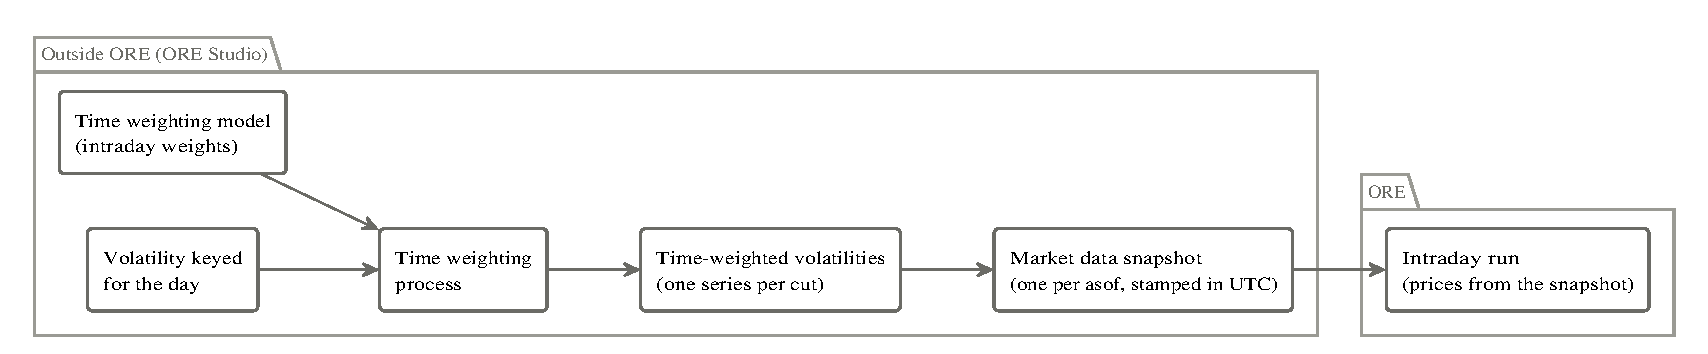
\includegraphics[width=\textwidth]{pics/time_weighting_flow.pdf}
\caption{Intraday time weighting outside ORE}
\label{fig:twflow}
\end{figure}

Section \ref{sec:ex-decay} demonstrates the approach with a time weighting process played by a script.

\subsection{The ATM and the Smile}\label{sec:atmsmile}

This document, its examples and its time weighting model concentrate on the ATM volatility. This subsection explains why, and
what this means for the rest of the smile.

\subsubsection*{Why the ATM Comes First}

In the last hours before a cut, gamma concentrates in a narrow band of strikes around spot. For a strike $K$ the gamma
of an option relative to the ATM option is about $\exp(-k^2/2)$, where $k$ is the distance from spot to strike in
standard deviations of the move left to the cut. Table \ref{tab:gammaconc} shows this for SP5 at 25\% volatility.

\begin{table}[H]
\centering
\begin{tabular}{|l|r|r|r|r|}
\hline
Time to cut & Standard deviation & \multicolumn{3}{c|}{Gamma relative to ATM} \\
 & index points & 0.25\% away & 0.5\% away & 1\% away \\
\hline
7 hours & 15.2 & 0.94 & 0.78 & 0.37 \\
1 hour & 5.7 & 0.65 & 0.17 & 0.001 \\
\hline
\end{tabular}
\caption{Concentration of gamma around the ATM strike, SP5 at 2147.56 and 25\% volatility}
\label{tab:gammaconc}
\end{table}

An hour before the cut, a strike 1\% from spot carries a thousandth of the ATM gamma. The headline gamma of a same day
options report therefore comes from options struck close to spot, and the volatility that drives it is the ATM
volatility. A further reason is data: for expiries within the day, quotes of the wings are thin, while the ATM
volatility is the quantity traders key and update through the day.

\subsubsection*{What ORE Supports}

Nothing in ORE is specific to the ATM. A volatility pillar at a cut is a pillar of the whole surface, and a snapshot can
carry any quotes the curve configuration accepts at that pillar:

\begin{itemize}
\item \textbf{Equity.} ATM quotes, as in the example of section \ref{sec:ex-decay}, or quotes by strike, since the
  equity volatility curve accepts wildcards in both expiries and strikes.
\item \textbf{FX.} ATM, risk reversal and butterfly quotes, or delta quotes, since the FX volatility curve accepts
  wildcard expiries for ATM, delta and risk reversal and butterfly curves, and FX quotes can carry an expiry at a cut
  (\textit{c.f.} section \ref{sec:fxfix}).
\item \textbf{Commodity.} ATM quotes with an expiry at a cut, as in the MultipleCutsCommodity example.
\end{itemize}

\subsubsection*{Risk Reversals and Butterflies}

How the smile of today's expiries moves through the day is a question for the time weighting model, not for ORE. Two treatments
are natural. Time-weighting only the ATM volatility, with risk reversals and butterflies held in volatility points relative to
it, shifts the smile in parallel as the ATM falls; it is simple, and it is a common way of rolling short dated
volatility. Scaling the whole smile with the ATM volatility shrinks the wings as well, which suits a smile that is
proportional to the level of volatility. The two differ mainly in the wings, which, as shown above, carry little of
the gamma within the day.

Time-weighting the risk reversals and butterflies is therefore future work for the time weighting model, with no change needed in ORE
beyond the FX expiry extension. Until then the time weighting process time-weights the ATM volatility and publishes the rest of the
smile of today's expiries as keyed, which ORE prices as it would any other quotes.

%-------------------------------------------------------------------------------
\section{Running the Report}\label{sec:setup}
%-------------------------------------------------------------------------------

This section collects the configuration of an intraday run of the same day options report.

\subsection{Market Configuration}

The market configuration should contain only what the options need: OIS discounting, equity and FX forward curves and
the volatility surfaces. Curves whose bootstrap instruments need past fixings fail at an intraday asof, see section
\ref{sec:limitations}.

\subsection{Sensitivity Configuration}

\begin{itemize}
\item \textbf{Short volatility pillars.} The sensitivity analysis reprices on the simulation market grid. Without 1D,
  1W and 1M expiries a one hour option is repriced with the vol of the first configured pillar. In a trial with a 6M
  first pillar the sensitivity base NPV was 1.51 against a pricing NPV of 1.16.
\item \textbf{Small spot shifts.} One hour before expiry the one standard deviation move of an equity index is a
  fraction of a percent, so a 1\% relative shift straddles the whole gamma peak. In a trial it gave a gamma of 19.1
  against a true value of 63.1. A relative shift of about one basis point is appropriate.
\item \textbf{Output precision.} Second order sensitivities to a one basis point shift are small numbers. Set
  \texttt{outputPrecision} to 8 or more.
\item \textbf{Additional results.} The \texttt{additionalResults} analytic reports the forward, volatility, discount
  factors and time to expiry used by the engine, which allows greeks to be checked against a closed form.
\end{itemize}

Section \ref{sec:examples} shows these settings at work in the examples.

\subsection{Pricing Engines}

American options priced by finite differences need time grids sized for hours to expiry. The SameDayInstruments
example uses at least 1000 time steps, 1000 grid points and 4 damping steps (\textit{c.f.} section \ref{sec:lim-fd}).

\subsection{Same Day Versions of ORE Studio Reports}\label{sec:reports}

ORE Studio's report catalogue \cite{orestudio} holds intraday reports that price from the live cut during the day, and
close twins that price at the end of the day. A same day version of a report runs the same report over the options
that expire on the valuation date, at an intraday asof, on the intraday build. Not every report needs one, and those
that do need different things from ORE. Table \ref{tab:reports} assesses the catalogue.

{\small
\begin{longtable}{|>{\raggedright\arraybackslash}p{3.6cm}|>{\raggedright\arraybackslash}p{1.6cm}|>{\raggedright\arraybackslash}p{8.0cm}|}
\hline
Report & Same day version & What it needs \\
\hline
\endfirsthead
\multicolumn{3}{l}{\textit{Table \ref{tab:reports}, continued}} \\
\hline
Report & Same day version & What it needs \\
\hline
\endhead
\multicolumn{3}{r}{\textit{continued on the next page}} \\
\endfoot
\endlastfoot
Headline Position & yes & Works with this document's approach: NPV and spot sensitivities with the volatility surface
not simulated. Vega needs a volatility shift at a cut. \\
\hline
Delta and gamma ladders & yes & Work. Spot shifts sized for hours to expiry rather than the usual 1\% (\textit{c.f.}
section \ref{sec:setup}). \\
\hline
Spot greeks (P\&L over a grid of spot levels) & yes & A grid of spot levels is a stress run; the stress analytic at
an intraday asof is untested. Repricing snapshots with spot shifted by ORE Studio works today. \\
\hline
Theta ladder & yes & A theta period of one day steps past today's cut. Needs a period of hours or minutes, or a
rerun at a later asof with that time's snapshot. \\
\hline
Vega ladders: ATM, risk reversal, butterfly, surface; triple vol spot ladder; volga; vanna & ATM vega and triple vol:
yes; others: low priority & Need volatility shifts at a cut, which the simulation market cannot provide (\textit{c.f.}
section \ref{sec:lim-simvol}). Snapshots with today's volatility quotes shifted by ORE Studio work today. \\
\hline
Intraday risk monitor & partly & PV and the delta ladder carry over. Parametric VaR on deltas and gammas is unsuitable
for options minutes from expiry; needs full revaluation over scenarios. \\
\hline
Intraday change & yes & Two intraday valuations, which the intraday build supports. Attribution should separate
intraday time weighting from market moves. \\
\hline
Spike, strike and option maps & yes & No pricing beyond deltas. The same day version buckets by cut rather than by
expiry date. \\
\hline
Spot ladder, DV01, rho, cross gamma, trades since last in & no & No same day option content. \\
\hline
Close twins of all reports & no & Today's options have expired by the close. \\
\hline
\end{longtable}
}
\vspace{-1.5em}
\begin{center}
\captionof{table}{Same day versions of ORE Studio's reports}\label{tab:reports}
\end{center}

The reports fall into three groups:

\begin{enumerate}
\item \textbf{Supported.} Headline position, the delta and gamma ladders, intraday change, and the PV and delta of the
  intraday risk monitor work with the approach of this document.
\item \textbf{To be verified.} Grids of spot levels need the stress analytic at an intraday asof, which has not been
  tested.
\item \textbf{To be built.} Volatility shifts at a cut for the vega reports (\textit{c.f.} section
  \ref{sec:lim-simvol}), theta periods within a day (\textit{c.f.} section \ref{sec:lim-theta}), and value at risk
  by full revaluation. Until they are built, the first two can be produced by ORE Studio repricing snapshots in which
  it has shifted the market data, one run per shift, in line with applying conventions before ORE.
\end{enumerate}

%-------------------------------------------------------------------------------
\section{Examples}\label{sec:examples}
%-------------------------------------------------------------------------------

The examples in \texttt{Examples/IntradayOptions} demonstrate the methodology of this document. They need the intraday
build and are not part of the default examples test suite. They are grouped by how the volatility for today's expiry
behaves through the day: flat in \texttt{FlatIntraday}, and set by intraday time weighting in \texttt{TimeWeighted}.

\subsection{Inventory}

\begin{table}[H]
\centering
\small
\begin{tabular}{|>{\raggedright\arraybackslash}p{4.3cm}|>{\raggedright\arraybackslash}p{4.3cm}|>{\raggedright\arraybackslash}p{3.6cm}|l|}
\hline
Example & Demonstrates & Main output & Section \\
\hline
\texttt{FlatIntraday/\allowbreak AtmGreeksToExpiry} & An ATM option valued through its last day, with greeks checked against the
closed form & \texttt{atm\_greeks.csv} & \ref{sec:ex-atm} \\
\hline
\texttt{FlatIntraday/\allowbreak SameDayInstruments} & Every instrument type in the scope of the report, priced
through the day and checked against closed forms or bounds & \texttt{same\_day\_\allowbreak instruments.csv} & \ref{sec:ex-instruments} \\
\hline
\texttt{TimeWeighted/}\newline\texttt{MultipleCutsFx},\newline\texttt{MultipleCutsEquity},\newline\texttt{MultipleCutsCommodity} & Several cuts in a day, each with its own time-weighted
volatility series, for FX, equity and commodity options & \texttt{multiple\_cuts\_\allowbreak *.csv}\newline
\texttt{published\_vols.csv} & \ref{sec:ex-multicuts} \\
\hline
\texttt{TimeWeighted/}\newline\texttt{TimeWeighted\allowbreak VersusFlat} & Pricing from an external series of time-weighted intraday volatilities, compared with a
flat volatility & \texttt{time\_weighted\_\allowbreak vs\_flat.csv}\newline \texttt{intraday\_vols.csv} & \ref{sec:ex-decay} \\
\hline
\end{tabular}
\caption{Intraday options examples}
\label{tab:inventory}
\end{table}

\subsection{Common Methodology}\label{sec:ex-method}

\subsubsection*{Layout}

Each example folder has the same layout:

\begin{itemize}
\item \texttt{run.py} runs the example and is the entry point of the examples test suite.
\item \texttt{run\_<name>.py} holds the steps of the example.
\item \texttt{Input/} holds \texttt{ore.xml} and the configuration specific to the example. Shared inputs, such as
  the end of day market data, fixings, conventions and pricing engines, come from \texttt{Examples/Input}.
\item \texttt{ExpectedOutput/} holds the reference results.
\end{itemize}

An example is run from its folder with \texttt{python run.py}, with the environment variable \texttt{ORE\_EXE}
pointing at the \texttt{ore} executable of the intraday build.

\subsubsection*{One Run per Asof}

Every example values the same trades at a series of asof times on one day. For each asof the script writes a market
data snapshot stamped with that time, as section \ref{sec:asofcuts} requires, writes a copy of \texttt{Input/ore.xml}
with the asof, the snapshot and an output folder \texttt{Output/T<hhmm>} filled in, and runs ORE on it. The script
then collects the results of all runs into one summary file. All times are UTC.

\subsubsection*{Independent Checks}

ORE's figures are checked against values computed outside ORE. The script reads the forward, volatility and discount
factors the engine used from the additional results report, and computes the Black-Scholes value and greeks from them.
Agreement shows that ORE's time to expiry and greeks are right, given the market the engine saw.

Greeks from ORE come from the sensitivity analysis. For a spot shift $h$ the report gives
$\Delta V_+ = V(S+h) - V(S)$ and $\Gamma_h = V(S+h) - 2V(S) + V(S-h)$. The scripts convert these to
$\Delta = (\Delta V_+ - \Gamma_h/2)/h$ and $\Gamma = \Gamma_h/h^2$. Shifts are one basis point relative, see
section \ref{sec:setup}.

\subsubsection*{Regression}

The files in \texttt{ExpectedOutput} are the reference results. The examples test suite compares them with a new run:

\begin{minted}[fontsize=\footnotesize]{text}
cd Examples
echo IntradayOptions/FlatIntraday/AtmGreeksToExpiry > list.txt
echo IntradayOptions/TimeWeighted/TimeWeightedVersusFlat >> list.txt
ORE_EXAMPLES_TEST_FILE=list.txt ORE_EXE=<intraday build>/App/ore \
    python run_examples_testsuite.py
\end{minted}

The suite prints \texttt{PyTest Return Code: 0} on success. It exits with zero whatever the result, see section
\ref{sec:lim-tooling}.

\subsection{FlatIntraday/AtmGreeksToExpiry}\label{sec:ex-atm}

\subsubsection*{Purpose}

With day resolution an option that expires today has a time to expiry of zero, so it is treated as expired or priced
at intrinsic value with zero gamma. The example shows that with intraday resolution ORE prices it with the remaining
time, and that its greeks behave as they should into the cut.

\subsubsection*{Inputs}

\begin{itemize}
\item An ATM SP5 call and put, strike equal to spot at 2147.56, expiring at 16:00 UTC on 5 February 2016, and a two
  year call with a date only expiry as a control.
\item The shared end of day market data and curve configuration, in which the SP5 volatility is 25\% at all expiries.
\item A market configuration with in currency OIS discounting only, so that no curve needs a past fixing, see section
  \ref{sec:limitations}.
\item A simulation market with short volatility pillars and a one basis point relative spot shift, as described in
  section \ref{sec:setup}.
\end{itemize}

\subsubsection*{Method}

ORE runs with NPV, additional results and sensitivity analytics at asof times from 09:00 to 15:59. The script writes
\texttt{atm\_greeks.csv} with the NPV, delta, gamma and vega of the call from ORE and from the closed form at each
time.

\subsubsection*{Checks}

\begin{enumerate}
\item The time to expiry in the NPV report is the remaining time, for example 0.000114 years, one hour, at 15:00.
\item NPV, delta and vega agree with the closed form.
\item Gamma grows as one over the square root of the time left, and vega and NPV fall as its square root.
\end{enumerate}

\subsubsection*{Results}

Table \ref{tab:atmevolution} shows the results.

\begin{table}[hbt]
\centering
\begin{tabular}{|l|r|r|r|r|r|r|}
\hline
Asof & Minutes left & NPV & Delta & Gamma ORE & Gamma closed form & Vega \\
\hline
09:00 & 420 & 6.050 & 0.5012 & 0.02629 & 0.02629 & 24.22 \\
12:00 & 240 & 4.574 & 0.5009 & 0.03477 & 0.03477 & 18.31 \\
14:00 & 120 & 3.235 & 0.5006 & 0.04917 & 0.04918 & 12.95 \\
15:00 & 60 & 2.288 & 0.5004 & 0.06954 & 0.06955 & 9.15 \\
15:30 & 30 & 1.618 & 0.5003 & 0.09833 & 0.09835 & 6.47 \\
15:45 & 15 & 1.144 & 0.5002 & 0.13903 & 0.13909 & 4.58 \\
15:55 & 5 & 0.661 & 0.5001 & 0.24058 & 0.24092 & 2.64 \\
15:59 & 1 & 0.295 & 0.5001 & 0.53496 & 0.53871 & 1.18 \\
\hline
\end{tabular}
\caption{ATM call expiring at 16:00, valued through the day}
\label{tab:atmevolution}
\end{table}

Figure \ref{fig:atmgamma} plots the gamma of table \ref{tab:atmevolution}. The closed form is evaluated at the same
asof times.

\begin{figure}[H]
\centering
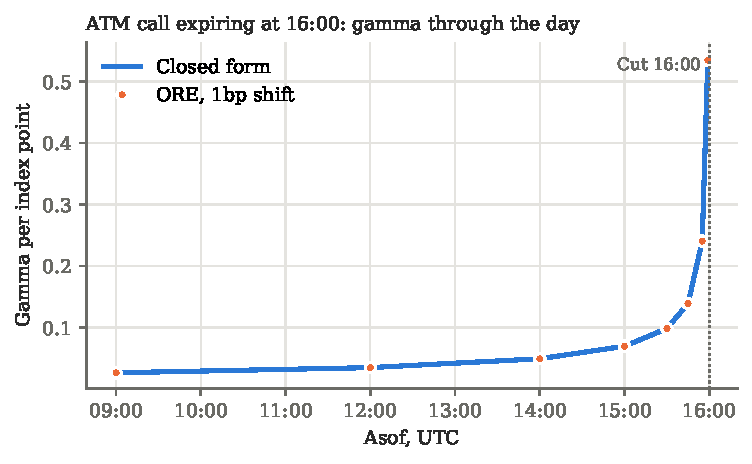
\includegraphics[width=0.85\textwidth]{pics/atm_gamma.pdf}
\caption{Gamma of the ATM call through its last day, ORE against the closed form}
\label{fig:atmgamma}
\end{figure}

\subsubsection*{What to Look For}

NPV, delta and vega agree with the closed form to five digits or more. Gamma grows from 0.026 at 09:00 to 0.535 at
15:59, a factor of about 20, which is $\sqrt{420}$. At 15:59 the finite difference gamma is 0.7\% low, because the one
basis point shift of 0.21 index points is already a third of the one minute standard deviation of 0.74 points. This is
a limit of the shift size. In the last minutes before the cut a smaller shift or the engine's analytic gamma should be
used.

\subsection{FlatIntraday/SameDayInstruments}\label{sec:ex-instruments}

\subsubsection*{Purpose}

The example extends \texttt{AtmGreeksToExpiry} to every instrument type in the scope of the same day options report
(\textit{c.f.} section \ref{sec:scope}). It shows that each type prices at an intraday asof with the remaining time to its own cut, and
that its value and greeks agree with a closed form or stay within bounds.

\subsubsection*{Inputs}

Eight trades expire on 5 February 2016 at the cut of their market:

\begin{itemize}
\item At 15:00 UTC, the New York 10:00 cut: a EURUSD call, a EURUSD cash-or-nothing digital call and a EURUSD one-touch
  with the barrier 0.5\% above spot, paid at expiry. A gold call also expires at 15:00 UTC, the time of the London
  afternoon gold price auction.
\item At 21:00 UTC, the SP5 close: an SP5 cash-or-nothing digital call, an SP5 up-and-out call with the barrier 1\%
  above spot, and an SP5 American put with a European put as its reference.
\end{itemize}

Each snapshot carries a EURUSD volatility pillar at the 15:00 UTC cut, held flat at today's level of 12.1699\%, so the
three FX trades are priced off a pillar at their own cut (\textit{c.f.} section \ref{sec:fxfix}). For the same reason the FX
volatilities are not simulated in the sensitivity analysis, and the example reports no FX vega (\textit{c.f.} section
\ref{sec:lim-simvol}). The base currency is USD, so that EURUSD shifts reach the simulation market. The example has its own pricing engine
configuration for the American put, see section \ref{sec:lim-fd}, and writes additional results with 12 digits, since
the default of 6 is too coarse for the checks of the digitals.

\subsubsection*{Method}

ORE runs at asof times from 09:00 to 20:55, including 14:55, five minutes before the FX cut, and 15:00, at the cut. The
script writes \texttt{same\_day\_instruments.csv} with one row per asof and trade.

\subsubsection*{Checks}

\begin{enumerate}
\item The time to expiry in the NPV report is the time to the trade's own cut.
\item NPV, delta and gamma agree with a closed form computed from the engine's forward, volatility and discount
  factors: Garman-Kohlhagen for the FX call, Black-76 for gold, cash-or-nothing formulas for the digitals, the
  Reiner-Rubinstein formula for the up-and-out call, the probability of a barrier hit, paid at expiry, for the
  one-touch, and Black-Scholes for the European put. The American put is compared with the European put, since the
  early exercise premium is negligible hours from expiry.
\item The up-and-out call is worth between zero and the vanilla call, and the one-touch between zero and its
  discounted payoff.
\end{enumerate}

Every greek is compared twice: with the exact derivative of the closed form, and with the closed form under ORE's own
one basis point shift. The second comparison separates an error of the shift from an error of the pricing.

\subsubsection*{Results}

The time to expiry matches the trade's cut in all 56 rows with a live trade. Table \ref{tab:instruments} shows the
largest differences over the asofs.

\begin{table}[H]
\centering
\footnotesize
\setlength{\tabcolsep}{4pt}
\begin{tabular}{|l|l|r|r|r|r|r|}
\hline
 & & NPV & \multicolumn{2}{c|}{Delta, relative} & \multicolumn{2}{c|}{Gamma, relative} \\
Trade & Reference & absolute & exact & same shift & exact & same shift \\
\hline
EURUSD call & Garman-Kohlhagen & $5\cdot10^{-7}$ & $7\cdot10^{-6}$ & $9\cdot10^{-8}$ & 0.59\% & $1.5\cdot10^{-6}$ \\
Gold call & Black-76 & $4\cdot10^{-7}$ & 5.7\% & $3\cdot10^{-7}$ & 1.07\% & $1.5\cdot10^{-6}$ \\
SP5 digital & cash-or-nothing & $5\cdot10^{-7}$ & 0.28\% & $5\cdot10^{-9}$ & 1.43\% & $1.7\cdot10^{-4}$ \\
EURUSD digital & cash-or-nothing & $5\cdot10^{-7}$ & 1.17\% & $1\cdot10^{-10}$ & 3.7\% & $1.9\cdot10^{-6}$ \\
SP5 up-and-out & Reiner-Rubinstein & $5\cdot10^{-7}$ & 0.09\% & $8\cdot10^{-6}$ & 0.14\% & $1.1\cdot10^{-5}$ \\
EURUSD one-touch & hit probability & $5\cdot10^{-7}$ & 5.7\% & $1.2\cdot10^{-4}$ & 2.5\% & $1.7\cdot10^{-5}$ \\
SP5 American put & European put & $2.8\cdot10^{-5}$ & $8\cdot10^{-6}$ & $5\cdot10^{-6}$ & 0.14\% & $2.3\cdot10^{-5}$ \\
SP5 European put & Black-Scholes & $5\cdot10^{-7}$ & $2\cdot10^{-6}$ & $5\cdot10^{-8}$ & 0.14\% & $3\cdot10^{-6}$ \\
\hline
\end{tabular}
\caption{SameDayInstruments: largest differences to the reference over the asofs}
\label{tab:instruments}
\end{table}

\subsubsection*{What to Look For}

\begin{itemize}
\item NPVs agree with their references to the six digits of the NPV report. The American put is worth at most
  $2.8\cdot10^{-5}$ more than the European put, and never less.
\item Against the exact derivatives, deltas and gammas differ by up to a few percent in the last minutes before a
  cut. Under the same shift the differences vanish, to $2\cdot10^{-4}$ or better, so they are errors of the one basis
  point shift, not of the pricing. Five minutes before the FX cut the shift is 0.27 standard deviations of EURUSD and
  0.36 of gold. Figure \ref{fig:bumperror} plots the relative gamma error against the exact closed form for every
  live trade and asof, against the size of the shift relative to the standard deviation of the move left to the cut.
  For the vanillas the error follows $0.1\,(h/\sigma_{\text{move}})^2$, the truncation error of a central second
  difference. The digitals, barrier and touch scatter above the line at small shifts, where their gamma is small and a
  small absolute difference is a large relative one.
\item Both bounds hold at every asof. The one-touch is worth 117 at 09:00 and 0.12 at 14:00. At 14:55 its barrier is 13
  standard deviations away, its value is zero and it has no sensitivity above the output threshold.
\item From 15:00, at and after their cut, the FX and gold trades are no longer in the NPV, additional results and
  sensitivity reports, see section \ref{sec:lim-matured}.
\end{itemize}

\begin{figure}[H]
\centering
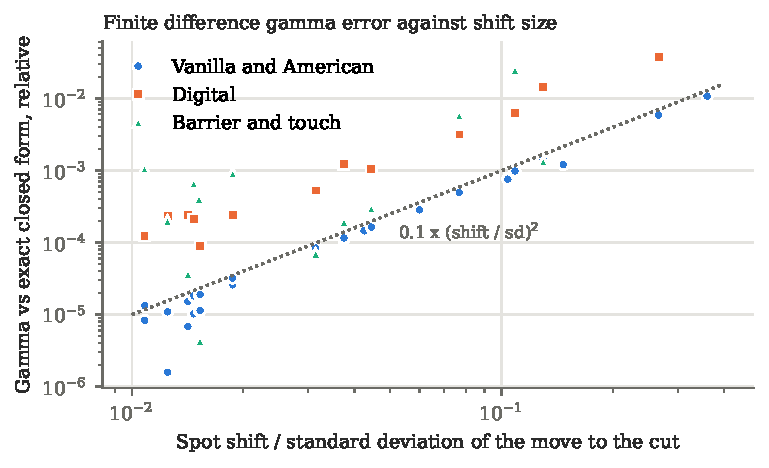
\includegraphics[width=0.85\textwidth]{pics/bump_error.pdf}
\caption{Relative gamma error of the one basis point shift against the exact closed form, by size of the shift relative to the remaining move, log scales}
\label{fig:bumperror}
\end{figure}

\subsection{TimeWeighted/MultipleCuts}\label{sec:ex-multicuts}

\subsubsection*{Purpose}

Three examples, \texttt{MultipleCutsFx}, \texttt{MultipleCutsEquity} and \texttt{MultipleCutsCommodity}, show the
market data model of section \ref{sec:mktdata} with several cuts in one day, one example per asset class. They show that
each option is priced off the volatility pillar at its own cut, with FX handled in the same way as equity and
commodity (\textit{c.f.} section \ref{sec:fxfix}).

\subsubsection*{Inputs}

\begin{itemize}
\item \textbf{FX.} EURUSD ATM calls expiring at the Tokyo cut, 06:00 UTC, the ECB cut, 13:30 UTC, and the New York cut,
  15:00 UTC.
\item \textbf{Equity.} SP5 ATM calls expiring at 14:30 UTC and at the close, 21:00 UTC.
\item \textbf{Commodity.} Gold ATM calls expiring at 10:30 UTC and 15:00 UTC.
\item In each example a control call expires a week later. Trades give a plain \texttt{ExerciseDate} and their cut as
  \texttt{ExpiryCutTime} in the envelope (\textit{c.f.} section \ref{sec:timezones}).
\end{itemize}

\subsubsection*{Method}

The examples share one script, \texttt{TimeWeighted/multiple\_cuts.py}, which plays the time weighting process. It applies the
variance time formulation of section \ref{sec:decay} with piecewise constant weights over the day, highest early and
lowest before the last cut, so that each cut's intraday time weightings. One weight profile serves all of a day's cuts, which
keeps total variance non-decreasing across them. For each asof the script publishes a snapshot with one volatility
pillar per cut that has not passed, and keyed tenor pillars beyond today; at some asofs it leaves the pillar of a passed
cut in the snapshot. ORE runs at each asof, and the script records, per trade, the volatility the engine used and the
NPV against the closed form.

\subsubsection*{Checks}

\begin{enumerate}
\item The volatility the engine reports for each trade equals the published volatility of its cut.
\item NPVs agree with the closed form computed from the engine's forward, volatility and discount factors.
\item A pillar for a cut that has passed is ignored, and an option past its cut leaves the reports.
\item Each cut's volatility falls through the day, and total variance does not decrease across a day's cuts.
\end{enumerate}

\subsubsection*{Results}

Tables \ref{tab:mcfx} to \ref{tab:mcco} show the published volatilities, and figure \ref{fig:multicutsfx} the EURUSD
series. Across the three examples the engine volatility equals the published volatility of the trade's cut to
$5\cdot 10^{-11}$, the rounding of the published quote, and NPVs agree with the closed form to $5\cdot 10^{-7}$, the
rounding of the NPV report. Passed pillars are logged as ignored, and options past their cut leave the reports.

\begin{table}[H]
\centering
\begin{tabular}{|l|r|r|r|}
\hline
Asof & 06:00 cut & 13:30 cut & 15:00 cut \\
\hline
03:00 & 14.55\% & 12.86\% & 12.53\% \\
05:55 & 13.47\% & 12.13\% & 11.79\% \\
09:00 & -- & 11.56\% & 11.17\% \\
12:00 & -- & 11.34\% & 10.65\% \\
13:25 & -- & 10.65\% & 9.96\% \\
14:00 & -- & -- & 9.53\% \\
14:55 & -- & -- & 8.25\% \\
\hline
\end{tabular}
\caption{MultipleCutsFx: published EURUSD ATM volatility per cut, UTC}
\label{tab:mcfx}
\end{table}

\begin{figure}[H]
\centering
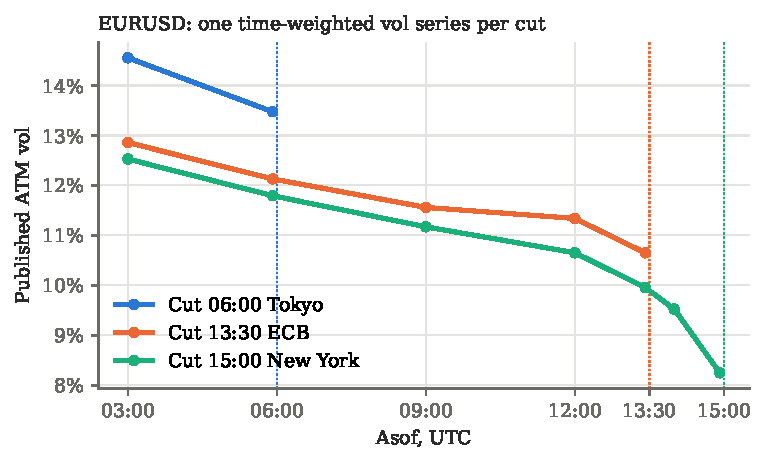
\includegraphics[width=0.85\textwidth]{pics/multi_cuts_fx.pdf}
\caption{MultipleCutsFx: the published volatility of each EURUSD cut through the day; dotted lines mark the cuts}
\label{fig:multicutsfx}
\end{figure}

\begin{table}[H]
\centering
\begin{tabular}{|l|r|r|}
\hline
Asof & 14:30 cut & 21:00 cut \\
\hline
03:00 & 17.94\% & 16.32\% \\
12:00 & 16.08\% & 13.91\% \\
14:25 & 14.68\% & 13.01\% \\
14:35 & -- & 12.96\% \\
17:00 & -- & 12.36\% \\
20:00 & -- & 11.21\% \\
20:55 & -- & 9.48\% \\
\hline
\end{tabular}
\caption{MultipleCutsEquity: published SP5 ATM volatility per cut, UTC}
\label{tab:mceq}
\end{table}

\begin{table}[H]
\centering
\begin{tabular}{|l|r|r|}
\hline
Asof & 10:30 cut & 15:00 cut \\
\hline
03:00 & 17.16\% & 15.64\% \\
08:00 & 15.58\% & 13.79\% \\
10:25 & 14.22\% & 12.72\% \\
10:45 & -- & 12.60\% \\
13:00 & -- & 11.61\% \\
14:55 & -- & 9.18\% \\
\hline
\end{tabular}
\caption{MultipleCutsCommodity: published gold ATM volatility per cut, UTC}
\label{tab:mcco}
\end{table}

\subsubsection*{What to Look For}

\begin{itemize}
\item Each cut has its own volatility at the same asof: at 03:00 the three EURUSD cuts are priced at different
  volatilities, which the tenor only surface of ORE before this work could not express.
\item Each series falls towards its cut, faster in the last hours, and the earlier cut's volatility stays above the
  later one's, as the decreasing weights imply.
\item The control call, expiring a week later, is priced off the keyed tenor pillars, with today's cut pillars entering
  only through interpolation.
\end{itemize}

\subsection{TimeWeighted/TimeWeightedVersusFlat}\label{sec:ex-decay}

\subsubsection*{Purpose}

The example shows ORE pricing an option that expires today from an intraday series of time-weighted volatilities, supplied
as market data, as described in section \ref{sec:decay}. Its script plays the part of the time weighting process.

\subsubsection*{Inputs}

\begin{itemize}
\item The underlying is SP5. The trading session runs from 14:30 to 21:00 UTC, 09:30 to 16:00 in New York. Today's cut
  is the close at 21:00 UTC.
\item At the open, 14:30 UTC, a volatility of 16\% is keyed for today's cut.
\item The weight $w(u)$ of an instant falls linearly from 2.0 at the open to 0.5 at the cut: the session is busiest
  after the open and quietest before the close.
\item Volatilities beyond today are keyed as usual and are not time-weighted: 12.71\% at 1M and 25\% at 6M.
\end{itemize}

With a linear weight the average weight over $[t, T]$ is $\bar w(t, T) = \frac{1}{2}\left(w(t) + w(T)\right)$, and the
variance time formulation of section \ref{sec:decay} reduces to
\begin{equation}
\sigma(t) = \sigma_0 \sqrt{\frac{\bar w(t, T)}{\bar w(t_0, T)}}
\end{equation}
The volatility for the remaining time is the keyed volatility, scaled by the square root of the average weight still
to come relative to the average weight of the whole session. It falls monotonically towards
$\sigma_0\sqrt{0.5/1.25} = 10.12\%$ at the cut. Table \ref{tab:decayseries} shows the intraday vols the time weighting process
generates.

\begin{table}[hbt]
\centering
\begin{tabular}{|l|r|}
\hline
Time (UTC) & Volatility \\
\hline
14:30 & 16.00\% \\
15:30 & 15.24\% \\
17:00 & 14.03\% \\
18:30 & 12.71\% \\
20:00 & 11.23\% \\
20:30 & 10.69\% \\
20:50 & 10.31\% \\
20:59 & 10.14\% \\
\hline
\end{tabular}
\caption{Intraday vols for today's cut}
\label{tab:decayseries}
\end{table}

The portfolio holds an ATM call expiring at today's cut and, as a control, an ATM call expiring at next week's cut.

\subsubsection*{Method}

For each time in the series the time weighting process writes a market data snapshot stamped with that time. It contains the
end of day market data, a volatility quote whose expiry is today's cut,
\texttt{EQUITY\_OPTION/RATE\_LNVOL/SP5/USD/2016-02-05T21:00/ATM/AtmFwd}, carrying the time-weighted value, and the keyed 1M
and 6M quotes. The SP5 volatility curve takes its pillars from the snapshot by wildcard. The pillar sits at today's cut
to confine the time weighting to today: a pillar at 1D would lie at the same time tomorrow, and options expiring tomorrow morning
would also take the time-weighted volatility.

Expiries after today and before the next pillar are interpolated in total variance between today's pillar and the
next pillar, so they still depend on today's quote. With 1M as the next pillar, an option expiring at next week's cut
puts a weight of about 0.76 on today's pillar. Today's total variance is small, $0.16^2 \cdot 4/8760 \approx 1.2\cdot
10^{-5}$ with four hours left, but so is the one week variance, about $3.2\cdot 10^{-4}$. Lowering today's volatility to
14\% changes the one week variance by about 0.6\%, and its volatility and NPV by about 0.3\%. Keyed pillars between
today and next week, such as 1D, remove the effect for later expiries.

The sensitivity analysis reprices on a simulation market. A simulated volatility surface is resampled onto expiry
tenors measured from the asof, which cannot hold a pillar at today's cut a few hours away: a one hour option would be
repriced with a volatility interpolated between the tenors, and the time weighting would be lost. In a first trial with a
simulated surface, the sensitivity base NPV at 17:00 was 2.337 against a pricing NPV of 2.566, and the time-weighted and flat
runs gave almost the same gamma. The example therefore does not simulate the SP5 volatilities. The simulation market
then wraps the pricing surface itself, the base NPV equals the pricing NPV, and spot shifts give the right gamma. The
cost is that the sensitivity analysis reports no vega, see section \ref{sec:lim-simvol}.

ORE runs at each time in the series twice, once with the time-weighted volatility and once with the volatility held at its
keyed value. The script collects the results in \texttt{time\_weighted\_vs\_flat.csv} and writes the series to
\texttt{intraday\_vols.csv}.

\subsubsection*{Checks}

\begin{enumerate}
\item \textbf{ORE prices from the series.} The volatility the engine reports in its additional results equals the
  time-weighted quote of the snapshot at every time. ORE has no knowledge of the time weighting model.
\item \textbf{Time weighting lowers the value of today's option.} With less variance left per remaining hour, the NPV with
  time weighting is below the NPV with the keyed volatility, and the gap widens through the session.
\item \textbf{Time weighting raises today's gamma.} ATM gamma is inversely proportional to $\sigma\sqrt{T}$, so at the same time
  the ratio of the gammas with and without time weighting is the ratio of the two volatilities.
\item \textbf{Today changes most.} The NPV of the control option moves only by the interpolation effect described
  above.
\end{enumerate}

\subsubsection*{Results and What to Look For}

Table \ref{tab:decayresults} shows the results. Gamma is from the sensitivity analysis with a one basis point relative
spot shift.

\begin{table}[hbt]
\centering
\footnotesize
\begin{tabular}{|l|r|r|r|r|r|r|r|r|}
\hline
 & & & \multicolumn{2}{c|}{NPV} & \multicolumn{2}{c|}{Gamma} & \multicolumn{2}{c|}{Control NPV} \\
Asof & Minutes & Vol & weighted & flat & weighted & flat & weighted & flat \\
\hline
14:30 & 390 & 16.00\% & 3.730 & 3.730 & 0.0426 & 0.0426 & 15.379 & 15.379 \\
15:30 & 330 & 15.24\% & 3.269 & 3.431 & 0.0486 & 0.0463 & 15.288 & 15.316 \\
17:00 & 240 & 14.03\% & 2.566 & 2.927 & 0.0619 & 0.0543 & 15.171 & 15.221 \\
18:30 & 150 & 12.71\% & 1.838 & 2.314 & 0.0865 & 0.0687 & 15.075 & 15.126 \\
20:00 & 60 & 11.23\% & 1.027 & 1.464 & 0.1548 & 0.1086 & 15.002 & 15.030 \\
20:30 & 30 & 10.69\% & 0.691 & 1.035 & 0.2298 & 0.1536 & 14.982 & 14.998 \\
20:50 & 10 & 10.31\% & 0.385 & 0.598 & 0.4113 & 0.2657 & 14.971 & 14.976 \\
20:59 & 1 & 10.14\% & 0.120 & 0.189 & 1.2745 & 0.8276 & 14.966 & 14.966 \\
\hline
\end{tabular}
\caption{ATM call expiring at today's cut, with time-weighted and flat volatility}
\label{tab:decayresults}
\end{table}

Figure \ref{fig:decay} shows the same runs. The volatility for today's cut falls through the session while the flat
volatility stays at its keyed value, the NPV with time weighting runs below the NPV without it, and the gamma with time weighting ends
above the gamma without it.

\begin{figure}[H]
\centering
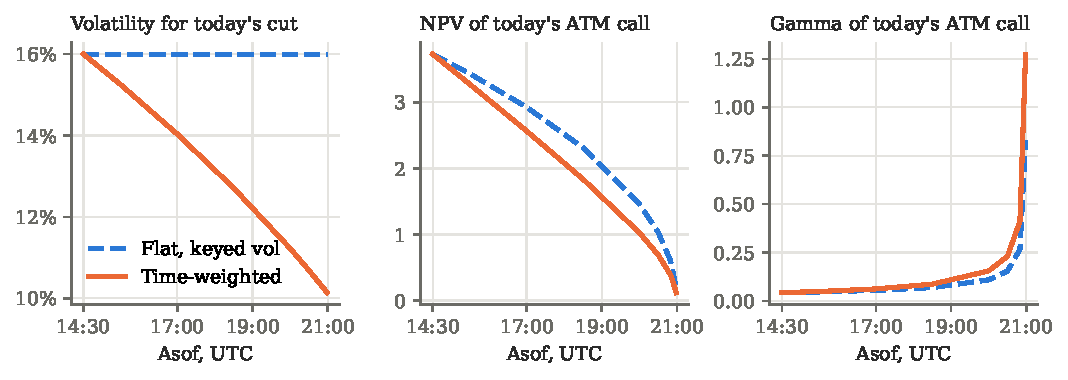
\includegraphics[width=1.0\textwidth]{pics/time_weighted_vs_flat.pdf}
\caption{Time-weighted against flat volatility through the session: the volatility for today's cut, and the NPV and gamma of the ATM call expiring at today's cut}
\label{fig:decay}
\end{figure}

\begin{enumerate}
\item The engine volatility equals the time-weighted quote at every time, to the six digits the report prints.
\item The NPV with time weighting falls below the NPV without it from the first step, and at 20:00 it is 30\% lower.
\item At 17:00 the gamma ratio is $0.0619/0.0543 = 1.14$, the ratio of the volatilities $16\%/14.03\% = 1.14$. The flat
  gamma, 0.0543, equals the closed form $\varphi(0)/(S\sigma\sqrt{T})$ at 16\% with four hours left. In the last minute
  the finite difference gamma with time weighting is 4\% below the closed form, 1.2745 against 1.328: at 10\% volatility the one
  basis point shift is 0.72 of the one minute standard deviation.
\item The control NPV differs by at most 0.34\%, at 18:30, from the interpolation effect. It does not differ at 14:30,
  when today's quote is the same in both runs, nor at 20:59, when today's pillar has almost no variance left.
\end{enumerate}

%-------------------------------------------------------------------------------
\section{Limitations}\label{sec:limitations}
%-------------------------------------------------------------------------------

The issues in sections \ref{sec:lim-fixingdates} to \ref{sec:lim-varswap} affect valuation at an intraday asof. The
same day options report as scoped in section \ref{sec:scope}, with a market configuration as described in section
\ref{sec:setup}, avoids them. The issues in sections \ref{sec:lim-matured} to \ref{sec:lim-serialization} do affect the
report. Section \ref{sec:lim-tooling} lists issues in the example and test tooling.

\subsection{Fixing Dates Derived from an Intraday Asof}\label{sec:lim-fixingdates}

\texttt{Calendar::advance} keeps the time of day, and \texttt{Index::pastFixing} looks up the fixing time series by
exact datetime. A date derived from a 15:00 asof, such as the asof moved back by one business day, is
2016-02-04T15:00. The fixing is stored at 2016-02-04T00:00, the lookup misses, and pricing fails with a missing fixing
error. Dates from a trade's own schedule are at midnight and are found. This affects for example curve bootstraps with
instruments that need past fixings.

\begin{minted}[fontsize=\footnotesize]{c++}
Settings::instance().evaluationDate() = Date(5, February, 2016, 15, 0, 0);
auto index = ext::make_shared<USDLibor>(3 * Months);
index->addFixing(Date(4, February, 2016), 0.006202);
index->fixing(Date(4, February, 2016)); // 0.006202
index->fixing(index->fixingCalendar().advance(
    Settings::instance().evaluationDate(), -1, Days)); // missing fixing
\end{minted}

The intended fix follows the rule of section \ref{sec:marketdata}: a fixing for day $D$ applies to the whole of $D$, so
a fixing date derived from an intraday asof is normalised to its day before the lookup.

\subsection{Today's Fixing Treated as Past}\label{sec:lim-todayfixing}

The \texttt{fixing()} methods of the indices compare the fixing date with the evaluation date. At a 15:00 asof today's
fixing date, at midnight, is earlier than the evaluation date, so the index requires a historical fixing instead of
forecasting it, and fails if none is available. The comparison should be made at day level for daily indices.

\subsection{Payments Dated Today}

\texttt{Event::hasOccurred} compares the event date with the evaluation date. A cashflow paying today is dated at
midnight, before a 15:00 evaluation date, so it counts as having occurred even when reference date events are
included. The settings \texttt{includeSettlementDateFlows} and \texttt{includeReferenceDateEvents} then have no effect,
and the cashflow is left out of the NPV without an error.

\subsection{Variance Swap Engine}\label{sec:lim-varswap}

The replicating variance swap engine, also used for volatility swaps, compares dates with the evaluation date
directly:

\begin{itemize}
\item The realised variance loop runs over all dates before the evaluation date. Today at midnight is earlier than
  15:00, so the loop asks for today's closing fixing, which does not exist yet, and the final return from spot then
  counts today a second time.
\item A swap starting today is not recognised as starting today.
\item A swap maturing today is valued at zero from the start of the day, although its final observation is at the
  close.
\end{itemize}

More generally, ORE compares dates with the evaluation date in several hundred places, each with an implicit
decision whether midnight today is in the past. Valuing products outside the scope of section \ref{sec:scope} at an
intraday asof requires a review of the comparisons on their pricing path.

\subsection{Options Past Their Cut}\label{sec:lim-matured}

Once the asof reaches an option's cut, ORE treats the trade as matured and leaves it out of the NPV, additional
results and sensitivity reports, with a warning in the log. A cash settled option that finished in the money is
therefore missing from the reports between its cut and its payment, although it is worth its payoff until paid. The
same day options report leaves such options out of its scope (\textit{c.f.} section \ref{sec:scope}).

\subsection{Finite Difference Settings for American Options}\label{sec:lim-fd}

The finite difference engine for American options sizes its time grid in steps per year, 100 in the shared pricing
engine configuration. With hours to expiry this gives a single time step, and the American put prices 23\% above its
European counterpart seven hours before the cut, with a negative gamma. More steps without damping overstate gamma by
60\%, and a finer spatial grid without damping prices the American below the European. The SameDayInstruments example
uses at least 1000 time steps, 1000 grid points, 4 damping steps and no monotone variance check, which gives a value at
most $2.8\cdot10^{-5}$ above the European put. A fixed grid point at $0.99/365$ years, which lies beyond expiry for an
option with less than a day to go, may contribute; this is not confirmed. The issue is not specific to intraday dates:
any option within a few days of expiry gets the single step grid. The intraday build makes it the normal case.

\subsection{Simulated Volatility Surfaces}\label{sec:lim-simvol}

The simulation market resamples a simulated volatility surface onto expiry tenors measured from the asof, such as
1D and 1W. A pillar at today's cut, a few hours from an intraday asof, cannot be represented on that grid. If the
surface carries such a pillar, as with time-weighted volatilities, the sensitivity analysis reprices same day options with an
interpolated volatility. Not simulating the surface keeps the pricing surface, but removes the surface from the
scenarios altogether: the sensitivity and stress analytics can then shift no volatility of that surface, at any expiry.
Vega, the volatility ladders and volatility stresses of a same day report are lost with it (\textit{c.f.} section
\ref{sec:reports}). They can be obtained by repricing market snapshots in which ORE Studio has shifted the volatility
quotes. Expiries given as datetimes in the simulation configuration would remove the limitation.

\subsection{Theta Within a Day}\label{sec:lim-theta}

The theta of the sensitivity analysis moves the valuation forward by a theta period, which is a tenor of at least one
day. For an option expiring at today's cut, a period of one day moves past its expiry, and the figure says nothing
about its time decay over the hours that remain. Theta within a day needs a period of hours or minutes, which ORE's tenors
do not express, or a rerun at a later asof with the snapshot of that time.

\subsection{XML Schema}\label{sec:lim-xsd}

The \texttt{date} type in \texttt{xsd/ore\_types.xsd} is limited to 10 characters, so schema validation rejects any
datetime, with or without a UTC offset. Trade XML is not affected, since expiry times go in the envelope as
\texttt{ExpiryCutTime} (\textit{c.f.} section \ref{sec:timezones}). A datetime written directly in \texttt{ExerciseDate} is still
accepted by the intraday build, but fails schema validation and the regular build, and should not be used.

\subsection{Serialization and Reporting}\label{sec:lim-serialization}

Date serialization stores the serial number only, so a datetime loses its time of day on a save and reload. Reports
print dates without the time of day, for example the maturity column of the NPV report. The maturity time column is
correct.

\subsection{Example and Test Tooling}\label{sec:lim-tooling}

The following issues were found while building and testing the examples. They are not specific to intraday dates.

\begin{itemize}
\item \textbf{Example test runner.} \texttt{Examples/run\_examples\_testsuite.py} prints the pytest return code but
  always exits with zero, so a failed run, or one that did not start, looks like a pass. It runs pytest with
  \texttt{-n 16}, which needs the \texttt{pytest-xdist} plugin. The file comparison in
  \texttt{Tools/PythonTools/compare\_files.py} uses the \texttt{Compare} class of \texttt{datacompy}, which was removed
  in \texttt{datacompy} 1.0. On Python 3.14, \texttt{datacompy} 0.16 installs with \texttt{-{}-no-deps}.
\item \textbf{Additional results report.} \texttt{additional\_results.csv} lists \texttt{strike} twice for each equity
  option, so trade id and result id do not form a unique key, and the example comparison fails on identical files. The
  Intraday Options example leaves this report out of its expected output.
\item \textbf{Derived schedule tests.} The OREData tests \texttt{ScheduleDataTests/testDerivedSchedules} open
  \texttt{./input/schedule/./input/schedule/derived\_schedules/...}, a doubled path, and fail. They fail in the default
  build too.
\end{itemize}

\subsection{Validation of This Work}\label{sec:lim-validation}

The evidence in this document rests on the following, and has the following limits.

\begin{itemize}
\item \textbf{Independence of the checks.} The changes to ORE, the examples, their checks and this document were
  developed with the help of an AI coding assistant, under the author's review (\textit{c.f.} section
  \ref{sec:aiuse}). A misunderstanding could therefore be carried consistently through code, checks and text, where
  checks written alongside the code would not detect it. Three things guard against this: the closed forms used in the
  checks are standard results, recomputed from the inputs the engine reports rather than from ORE's own greeks;
  QuantLib's tests of its high resolution dates are upstream and independent of this work; and existing ORE results,
  such as Legacy Example 22, are reproduced unchanged.
\item \textbf{Regression.} The expected outputs of the examples were produced by the same runs that they now check.
  They detect a change in results, not an error that was present when they were produced.
\item \textbf{Data.} The examples use ORE's example market data of 5 February 2016 and an illustrative time weighting model, not
  intraday market data observed through a trading day.
\item \textbf{Use in production.} The same day options report has not yet been run in ORE Studio (\textit{c.f.}
  section \ref{sec:orestudio}).
\end{itemize}

%-------------------------------------------------------------------------------
\section{Conclusion}\label{sec:conclusion}
%-------------------------------------------------------------------------------

\subsection{Findings}

\begin{itemize}
\item \textbf{Day resolution cannot value same day options.} An option that expires on the valuation date has a time
  to expiry of zero, so it is valued as expired or at intrinsic value, with no gamma, at the point of its life where
  gamma is largest.
\item \textbf{An intraday build solves this without changes to the pricing code.} With
  \texttt{QL\_HIGH\_RESOLUTION\_DATE}, the time to expiry is the remaining time, and the day counters, volatility
  surfaces and pricing engines of QuantLib and ORE use it as they are. No pricing model or engine changes. The
  changes to ORE are confined to its inputs and market construction: date input accepts a time of day and a UTC
  offset; option data reads an optional expiry cut time from the trade's envelope, so one trade XML serves both
  builds; and FX volatility quotes accept an expiry date or datetime, so that FX surfaces can have a pillar at a cut,
  as equity surfaces already can.
\item \textbf{The intraday build is as stable as the default build on day resolution inputs.} It compiles without
  errors, passes the unit tests that pass in the default build, and reproduces the expected output of an existing
  example to $3\cdot 10^{-14}$. It is somewhat slower.
\item \textbf{The greeks are right.} For an ATM option valued through its last day, NPV, delta and vega agree with the
  Black-Scholes closed form to five digits or more, and gamma grows as $1/\sqrt{T}$ into the cut. Every instrument
  type in the scope of the report, FX and gold vanillas, digitals, a barrier, a one-touch and an American option,
  prices with the remaining time to its own cut and agrees with a closed form or stays within bounds, without changes to
  the pricing code. The American option needs finer finite difference settings than the default. With several cuts in
  a day, FX, equity and commodity options each price off the volatility pillar at their own cut.
\item \textbf{Time and volatility conventions stay outside ORE.} ORE prices from UTC timestamps and from the
  volatilities a market snapshot carries. Cuts are converted to UTC by the booking system, and intraday time weighting is
  produced by an external process. The time weighting example shows ORE pricing from a time-weighted series, with the weighting confined to
  today's expiry by a volatility pillar at today's cut.
\end{itemize}

\subsection{Recommendations for the Same Day Options Report}

\begin{enumerate}
\item Build and deploy the intraday build separately from the regular build, and use it only for the same day options
  report. Value all other trades with the regular build.
\item Restrict the report to the instruments of section \ref{sec:scope}, and reject other trade types when the asof
  carries a time.
\item Stamp every market data snapshot, and the asof, with the valuation time in UTC.
\item Give option expiries as a plain \texttt{ExerciseDate} and the cut, converted to UTC, as \texttt{ExpiryCutTime}
  in the trade's envelope, for every option, whichever build the report targets.
\item Keep the market configuration to the curves and surfaces options need, with in currency OIS discounting, so that
  no curve needs a past fixing.
\item Configure the sensitivity analysis for short expiries: short volatility pillars, a one basis point relative spot
  shift and an output precision of 8. With a volatility pillar at today's cut, do not simulate the volatility surface.
\item Produce time-weighted volatilities in the market data process, with a pillar at today's cut.
\item Set \texttt{EnforceMonotoneVariance} on FX volatility curves that carry pillars at today's cuts, so that an
  inconsistent snapshot fails rather than prices, in addition to ORE Studio's own check.
\item Price American options with finite difference settings sized for hours to expiry, as in the SameDayInstruments
  example, see section \ref{sec:lim-fd}.
\end{enumerate}

\subsection{Open Items}

\begin{itemize}
\item \textbf{Same day report capabilities.} Test the stress analytic at an intraday asof, for grids of spot levels;
  support volatility shifts at a cut and theta periods within a day; and use value at risk by full revaluation for
  same day options (\textit{c.f.} section \ref{sec:reports}).
\item \textbf{Validation in ORE Studio.} Package the intraday build for the ORE Studio compute grid, run the same day
  options report there, and add the evidence to this document (\textit{c.f.} section \ref{sec:orestudio}).
\item \textbf{Vega to today's pillar.} With the surface not simulated, the sensitivity analysis reports no vega. Either
  the time weighting process reprices a snapshot with today's quote shifted, or the simulation configuration learns expiries
  given as datetimes. See section \ref{sec:lim-simvol}.
\item \textbf{Reports.} Dates in reports are printed without the time of day, and serialization drops it. See section
  \ref{sec:lim-serialization}.
\item \textbf{Wider use of an intraday asof.} Valuing anything beyond the report's scope at an intraday asof needs the
  daily fixing and payment rules of section \ref{sec:marketdata} and a review of the date comparisons on each pricing
  path. See sections \ref{sec:lim-fixingdates} to \ref{sec:lim-varswap}.
\item \textbf{Settlement fixings at a cut.} Options that expired earlier today and await their settlement fixing
  need the valuation date rule of section \ref{sec:marketdata} for their fixing source, which ORE does not yet apply
  consistently at an intraday asof.
\end{itemize}

\begin{thebibliography}{5}

\bibitem{fpmlfxexercise} FpML: complex type FxEuropeanExercise, with \texttt{expiryDate}, \texttt{expiryTime} and
  \texttt{cutName}, FpML 5.8 confirmation view,
  \url{https://www.fpml.org/spec/fpml-5-8-9-rec-2/html/confirmation/schemaDocumentation/schemas/fpml-fx-5-8_xsd/complexTypes/FxEuropeanExercise.html}

\bibitem{fpmlcutname} FpML: cut name coding scheme, version 1-0, \url{https://www.fpml.org/coding-scheme/cut-name}

\bibitem{quantlib} QuantLib: a free/open source library for quantitative finance, \url{https://www.quantlib.org}

\bibitem{ore} Open Source Risk Engine (ORE), \url{https://www.opensourcerisk.org}

\bibitem{qlhighres} Spanderen, Klaus: preprocessor directive to toggle between the existing date class and a high
  resolution datetime class, QuantLib commit f5b2d8f, 12 August 2015,
  \url{https://github.com/lballabio/QuantLib/commit/f5b2d8f7efe65d39007f126cc982529c531f7ba1}

\bibitem{orestudio} ORE Studio: a graphical front end for the Open Source Risk Engine,
  \url{https://github.com/OreStudio/OreStudio}

\bibitem{andersen1997} Andersen, Torben G., and Bollerslev, Tim: Intraday Periodicity and Volatility Persistence in
  Financial Markets, Journal of Empirical Finance 4, 115--158, 1997

\bibitem{andersen1998} Andersen, Torben G., and Bollerslev, Tim: Deutsche Mark--Dollar Volatility: Intraday Activity
  Patterns, Macroeconomic Announcements, and Longer Run Dependencies, Journal of Finance 53, 219--265, 1998.
  NBER Working Paper 5752, \url{https://www.nber.org/papers/w5752}

\bibitem{clark2011} Clark, Iain J.: Foreign Exchange Option Pricing: A Practitioner's Guide, Wiley, 2011.
  Tables 4.7 and 4.8, sample short dated EURUSD day weights and intraday weights

\bibitem{globalcapital} GlobalCapital: Pricing Short Dated Options,
  \url{https://www.globalcapital.com/article/28mwtvkodfvd095dm36yo/derivatives/pricing-short-dated-options}

\bibitem{moontower} Moontower: Weekend Theta, \url{https://moontowermeta.com/weekend-theta/}

\bibitem{wright2020} Wright, Jonathan H.: Event-Day Options, NBER Working Paper 28306, December 2020,
  \url{https://www.nber.org/papers/w28306}

\end{thebibliography}

\end{document}
